\documentclass[twoside]{book}

% Packages required by doxygen
\usepackage{fixltx2e}
\usepackage{calc}
\usepackage{doxygen}
\usepackage[export]{adjustbox} % also loads graphicx
\usepackage{graphicx}
\usepackage[utf8]{inputenc}
\usepackage{makeidx}
\usepackage{multicol}
\usepackage{multirow}
\PassOptionsToPackage{warn}{textcomp}
\usepackage{textcomp}
\usepackage[nointegrals]{wasysym}
\usepackage[table]{xcolor}

% Font selection
\usepackage[T1]{fontenc}
\usepackage[scaled=.90]{helvet}
\usepackage{courier}
\usepackage{amssymb}
\usepackage{sectsty}
\renewcommand{\familydefault}{\sfdefault}
\allsectionsfont{%
  \fontseries{bc}\selectfont%
  \color{darkgray}%
}
\renewcommand{\DoxyLabelFont}{%
  \fontseries{bc}\selectfont%
  \color{darkgray}%
}
\newcommand{\+}{\discretionary{\mbox{\scriptsize$\hookleftarrow$}}{}{}}

% Page & text layout
\usepackage{geometry}
\geometry{%
  a4paper,%
  top=2.5cm,%
  bottom=2.5cm,%
  left=2.5cm,%
  right=2.5cm%
}
\tolerance=750
\hfuzz=15pt
\hbadness=750
\setlength{\emergencystretch}{15pt}
\setlength{\parindent}{0cm}
\setlength{\parskip}{3ex plus 2ex minus 2ex}
\makeatletter
\renewcommand{\paragraph}{%
  \@startsection{paragraph}{4}{0ex}{-1.0ex}{1.0ex}{%
    \normalfont\normalsize\bfseries\SS@parafont%
  }%
}
\renewcommand{\subparagraph}{%
  \@startsection{subparagraph}{5}{0ex}{-1.0ex}{1.0ex}{%
    \normalfont\normalsize\bfseries\SS@subparafont%
  }%
}
\makeatother

% Headers & footers
\usepackage{fancyhdr}
\pagestyle{fancyplain}
\fancyhead[LE]{\fancyplain{}{\bfseries\thepage}}
\fancyhead[CE]{\fancyplain{}{}}
\fancyhead[RE]{\fancyplain{}{\bfseries\leftmark}}
\fancyhead[LO]{\fancyplain{}{\bfseries\rightmark}}
\fancyhead[CO]{\fancyplain{}{}}
\fancyhead[RO]{\fancyplain{}{\bfseries\thepage}}
\fancyfoot[LE]{\fancyplain{}{}}
\fancyfoot[CE]{\fancyplain{}{}}
\fancyfoot[RE]{\fancyplain{}{\bfseries\scriptsize Generated by Doxygen }}
\fancyfoot[LO]{\fancyplain{}{\bfseries\scriptsize Generated by Doxygen }}
\fancyfoot[CO]{\fancyplain{}{}}
\fancyfoot[RO]{\fancyplain{}{}}
\renewcommand{\footrulewidth}{0.4pt}
\renewcommand{\chaptermark}[1]{%
  \markboth{#1}{}%
}
\renewcommand{\sectionmark}[1]{%
  \markright{\thesection\ #1}%
}

% Indices & bibliography
\usepackage{natbib}
\usepackage[titles]{tocloft}
\setcounter{tocdepth}{3}
\setcounter{secnumdepth}{5}
\makeindex

% Hyperlinks (required, but should be loaded last)
\usepackage{ifpdf}
\ifpdf
  \usepackage[pdftex,pagebackref=true]{hyperref}
\else
  \usepackage[ps2pdf,pagebackref=true]{hyperref}
\fi
\hypersetup{%
  colorlinks=true,%
  linkcolor=blue,%
  citecolor=blue,%
  unicode%
}

% Custom commands
\newcommand{\clearemptydoublepage}{%
  \newpage{\pagestyle{empty}\cleardoublepage}%
}

\usepackage{caption}
\captionsetup{labelsep=space,justification=centering,font={bf},singlelinecheck=off,skip=4pt,position=top}

%===== C O N T E N T S =====

\begin{document}

% Titlepage & ToC
\hypersetup{pageanchor=false,
             bookmarksnumbered=true,
             pdfencoding=unicode
            }
\pagenumbering{alph}
\begin{titlepage}
\vspace*{7cm}
\begin{center}%
{\Large My Project }\\
\vspace*{1cm}
{\large Generated by Doxygen 1.8.14}\\
\end{center}
\end{titlepage}
\clearemptydoublepage
\pagenumbering{roman}
\tableofcontents
\clearemptydoublepage
\pagenumbering{arabic}
\hypersetup{pageanchor=true}

%--- Begin generated contents ---
\chapter{Hierarchical Index}
\section{Class Hierarchy}
This inheritance list is sorted roughly, but not completely, alphabetically\+:\begin{DoxyCompactList}
\item \contentsline{section}{Painter}{\pageref{class_painter}}{}
\begin{DoxyCompactList}
\item \contentsline{section}{Actor}{\pageref{class_actor}}{}
\begin{DoxyCompactList}
\item \contentsline{section}{Ghost}{\pageref{class_ghost}}{}
\item \contentsline{section}{Pacman}{\pageref{class_pacman}}{}
\end{DoxyCompactList}
\item \contentsline{section}{Tile}{\pageref{class_tile}}{}
\end{DoxyCompactList}
\item Q\+Main\+Window\begin{DoxyCompactList}
\item \contentsline{section}{Main\+Window}{\pageref{class_main_window}}{}
\end{DoxyCompactList}
\item Q\+Widget\begin{DoxyCompactList}
\item \contentsline{section}{clientwindow}{\pageref{classclientwindow}}{}
\item \contentsline{section}{game\+Options}{\pageref{classgame_options}}{}
\item \contentsline{section}{game\+Window}{\pageref{classgame_window}}{}
\item \contentsline{section}{server\+Window}{\pageref{classserver_window}}{}
\end{DoxyCompactList}
\end{DoxyCompactList}

\chapter{Class Index}
\section{Class List}
Here are the classes, structs, unions and interfaces with brief descriptions\+:\begin{DoxyCompactList}
\item\contentsline{section}{\mbox{\hyperlink{class_actor}{Actor}} }{\pageref{class_actor}}{}
\item\contentsline{section}{\mbox{\hyperlink{classclientwindow}{clientwindow}} }{\pageref{classclientwindow}}{}
\item\contentsline{section}{\mbox{\hyperlink{classgame_options}{game\+Options}} }{\pageref{classgame_options}}{}
\item\contentsline{section}{\mbox{\hyperlink{classgame_window}{game\+Window}} }{\pageref{classgame_window}}{}
\item\contentsline{section}{\mbox{\hyperlink{class_ghost}{Ghost}} }{\pageref{class_ghost}}{}
\item\contentsline{section}{\mbox{\hyperlink{class_main_window}{Main\+Window}} }{\pageref{class_main_window}}{}
\item\contentsline{section}{\mbox{\hyperlink{class_pacman}{Pacman}} }{\pageref{class_pacman}}{}
\item\contentsline{section}{\mbox{\hyperlink{class_painter}{Painter}} }{\pageref{class_painter}}{}
\item\contentsline{section}{\mbox{\hyperlink{classserver_window}{server\+Window}} }{\pageref{classserver_window}}{}
\item\contentsline{section}{\mbox{\hyperlink{class_tile}{Tile}} }{\pageref{class_tile}}{}
\end{DoxyCompactList}

\chapter{File Index}
\section{File List}
Here is a list of all documented files with brief descriptions\+:\begin{DoxyCompactList}
\item\contentsline{section}{\mbox{\hyperlink{actor_8cpp}{actor.\+cpp}} }{\pageref{actor_8cpp}}{}
\item\contentsline{section}{{\bfseries actor.\+h} }{\pageref{actor_8h}}{}
\item\contentsline{section}{\mbox{\hyperlink{clientwindow_8cpp}{clientwindow.\+cpp}} }{\pageref{clientwindow_8cpp}}{}
\item\contentsline{section}{{\bfseries clientwindow.\+h} }{\pageref{clientwindow_8h}}{}
\item\contentsline{section}{{\bfseries game\+\_\+cfg.\+h} }{\pageref{game__cfg_8h}}{}
\item\contentsline{section}{\mbox{\hyperlink{gameoptions_8cpp}{gameoptions.\+cpp}} }{\pageref{gameoptions_8cpp}}{}
\item\contentsline{section}{{\bfseries gameoptions.\+h} }{\pageref{gameoptions_8h}}{}
\item\contentsline{section}{\mbox{\hyperlink{gamewindow_8cpp}{gamewindow.\+cpp}} }{\pageref{gamewindow_8cpp}}{}
\item\contentsline{section}{{\bfseries gamewindow.\+h} }{\pageref{gamewindow_8h}}{}
\item\contentsline{section}{\mbox{\hyperlink{ghost_8cpp}{ghost.\+cpp}} }{\pageref{ghost_8cpp}}{}
\item\contentsline{section}{{\bfseries ghost.\+h} }{\pageref{ghost_8h}}{}
\item\contentsline{section}{{\bfseries globaltypes.\+h} }{\pageref{globaltypes_8h}}{}
\item\contentsline{section}{\mbox{\hyperlink{main_8cpp}{main.\+cpp}} }{\pageref{main_8cpp}}{}
\item\contentsline{section}{\mbox{\hyperlink{mainwindow_8cpp}{mainwindow.\+cpp}} }{\pageref{mainwindow_8cpp}}{}
\item\contentsline{section}{{\bfseries mainwindow.\+h} }{\pageref{mainwindow_8h}}{}
\item\contentsline{section}{\mbox{\hyperlink{pacman_8cpp}{pacman.\+cpp}} }{\pageref{pacman_8cpp}}{}
\item\contentsline{section}{{\bfseries pacman.\+h} }{\pageref{pacman_8h}}{}
\item\contentsline{section}{\mbox{\hyperlink{painter_8cpp}{painter.\+cpp}} }{\pageref{painter_8cpp}}{}
\item\contentsline{section}{{\bfseries painter.\+h} }{\pageref{painter_8h}}{}
\item\contentsline{section}{\mbox{\hyperlink{serverwindow_8h}{serverwindow.\+h}} }{\pageref{serverwindow_8h}}{}
\item\contentsline{section}{\mbox{\hyperlink{tile_8cpp}{tile.\+cpp}} }{\pageref{tile_8cpp}}{}
\item\contentsline{section}{{\bfseries tile.\+h} }{\pageref{tile_8h}}{}
\end{DoxyCompactList}

\chapter{Class Documentation}
\hypertarget{class_actor}{}\section{Actor Class Reference}
\label{class_actor}\index{Actor@{Actor}}


{\ttfamily \#include $<$actor.\+h$>$}

Inheritance diagram for Actor\+:\begin{figure}[H]
\begin{center}
\leavevmode
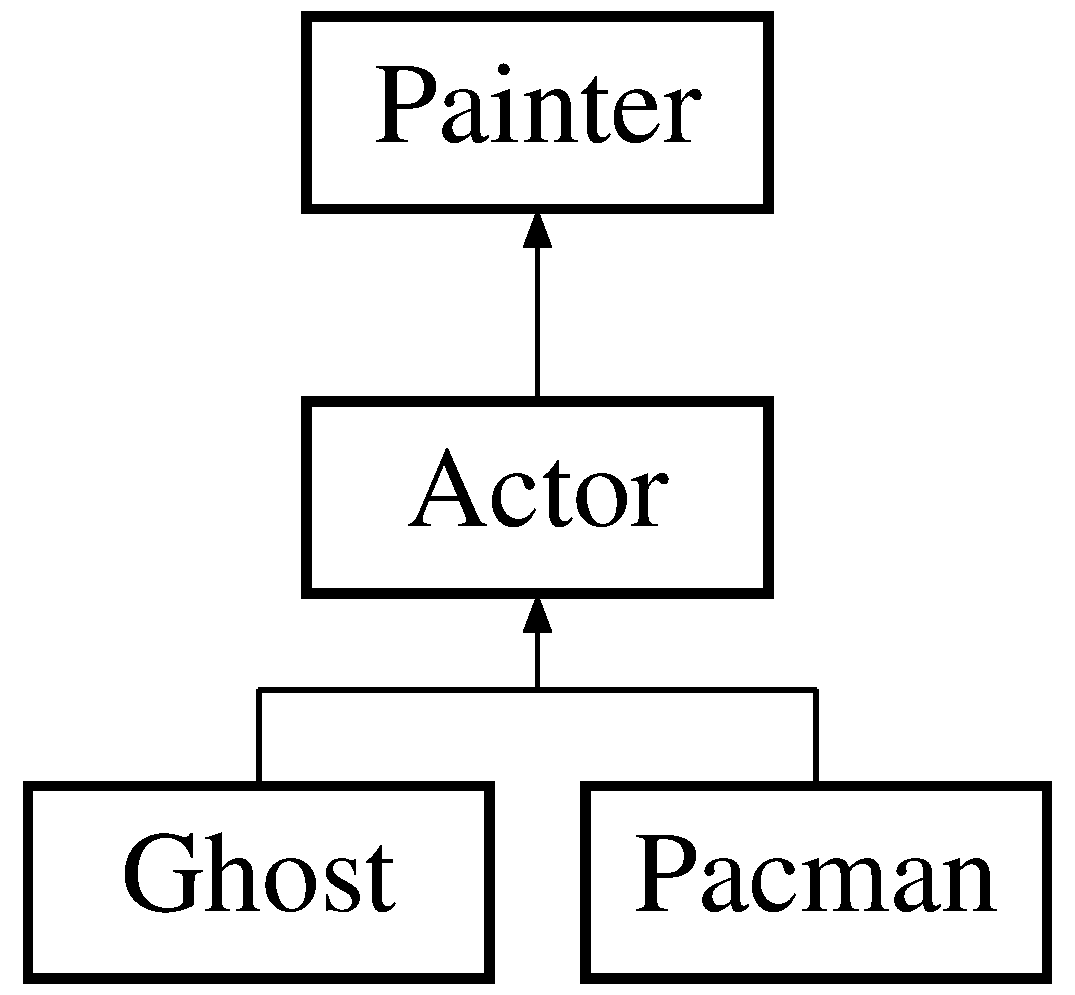
\includegraphics[height=3.000000cm]{class_actor}
\end{center}
\end{figure}
\subsection*{Public Member Functions}
\begin{DoxyCompactItemize}
\item 
\mbox{\hyperlink{class_actor_a2a0ff4335a1ee9096df90f288c026c8b}{Actor}} ()
\begin{DoxyCompactList}\small\item\em Empty actor class constructor. \end{DoxyCompactList}\item 
\mbox{\hyperlink{class_actor_a651899b4ab39be662d785c298a2a2fae}{Actor}} (Q\+String pixmap\+Path, int x, int y)
\begin{DoxyCompactList}\small\item\em Overloaded actor class constructor. \end{DoxyCompactList}\item 
int \mbox{\hyperlink{class_actor_aa24a5fe0a46ca8274d993f7fe2954aa5}{get\+Curr\+Tile}} () const
\begin{DoxyCompactList}\small\item\em curr\+Tile getter. \end{DoxyCompactList}\item 
void \mbox{\hyperlink{class_actor_a0e9374b0779e9b79af21278a4698a138}{update\+Curr\+Tile}} (void)
\begin{DoxyCompactList}\small\item\em updates curr\+Tile (current tile) based on x and y positions. \end{DoxyCompactList}\item 
void \mbox{\hyperlink{class_actor_a66e25276468e157b822c9df798eb3e6a}{move\+Left}} (void)
\begin{DoxyCompactList}\small\item\em Changes \mbox{\hyperlink{class_actor}{Actor}} x position by T\+I\+L\+E\+\_\+\+W\+I\+D\+TH to the left. \end{DoxyCompactList}\item 
void \mbox{\hyperlink{class_actor_a66a756cd694913854af20352d4f0bedd}{move\+Right}} (void)
\begin{DoxyCompactList}\small\item\em Changes \mbox{\hyperlink{class_actor}{Actor}} x position by T\+I\+L\+E\+\_\+\+W\+I\+D\+TH to the right. \end{DoxyCompactList}\item 
void \mbox{\hyperlink{class_actor_a096be226cbfb42f7595283703742da89}{move\+Up}} (void)
\begin{DoxyCompactList}\small\item\em Changes \mbox{\hyperlink{class_actor}{Actor}} y position by T\+I\+L\+E\+\_\+\+H\+E\+I\+G\+HT upwords. \end{DoxyCompactList}\item 
void \mbox{\hyperlink{class_actor_abc0ed5cc187310fef30b4b9a94252e17}{move\+Down}} (void)
\begin{DoxyCompactList}\small\item\em Changes \mbox{\hyperlink{class_actor}{Actor}} y position by T\+I\+L\+E\+\_\+\+H\+E\+I\+G\+HT downwards. \end{DoxyCompactList}\item 
int \mbox{\hyperlink{class_actor_a0f751e7ea9030b58a8db19ccc62214f3}{get\+Tile\+Index\+Left}} () const
\begin{DoxyCompactList}\small\item\em Returns position of the tile left to the \mbox{\hyperlink{class_actor}{Actor}}. \end{DoxyCompactList}\item 
int \mbox{\hyperlink{class_actor_ac54394e212a1a1f51ae82202a8144421}{get\+Tile\+Index\+Right}} () const
\begin{DoxyCompactList}\small\item\em Returns position of the tile right to the \mbox{\hyperlink{class_actor}{Actor}}. \end{DoxyCompactList}\item 
int \mbox{\hyperlink{class_actor_a92a718240f1b2b51e2f0dee763435f58}{get\+Tile\+Index\+Up}} () const
\begin{DoxyCompactList}\small\item\em Returns position of the tile upwards to the \mbox{\hyperlink{class_actor}{Actor}}. \end{DoxyCompactList}\item 
int \mbox{\hyperlink{class_actor_a78388b58a561143504ff722a6625b564}{get\+Tile\+Index\+Down}} () const
\begin{DoxyCompactList}\small\item\em Returns position of the tile downwards to the \mbox{\hyperlink{class_actor}{Actor}}. \end{DoxyCompactList}\item 
int \mbox{\hyperlink{class_actor_a7867adac1be8ea6273808dda395a4170}{get\+Last\+Tile}} () const
\begin{DoxyCompactList}\small\item\em last\+Tile getter. \end{DoxyCompactList}\item 
void \mbox{\hyperlink{class_actor_a4d708f5e042cd6558947820f33520d61}{set\+Last\+Tile}} (int value)
\begin{DoxyCompactList}\small\item\em last\+Tile setter. \end{DoxyCompactList}\item 
int \mbox{\hyperlink{class_actor_ab50ceeaf6192f75be8ed9b41d8c585fb}{get\+Speed}} () const
\begin{DoxyCompactList}\small\item\em speed getter. \end{DoxyCompactList}\item 
void \mbox{\hyperlink{class_actor_aa678f8ed8724d19bd309e88b1e130840}{set\+Speed}} (int value)
\begin{DoxyCompactList}\small\item\em speed setter. \end{DoxyCompactList}\item 
int \mbox{\hyperlink{class_actor_a20bb92df0514cc00b31cb1a046548964}{get\+Direction}} () const
\begin{DoxyCompactList}\small\item\em direction getter. \end{DoxyCompactList}\item 
void \mbox{\hyperlink{class_actor_ad0049dcc53c477e38400b0c41536c51a}{set\+Direction}} (int value)
\begin{DoxyCompactList}\small\item\em direction setter. \end{DoxyCompactList}\end{DoxyCompactItemize}
\subsection*{Additional Inherited Members}


\subsection{Detailed Description}
\mbox{\hyperlink{class_actor}{Actor}} class is responsible for moving and controlling all Actors (\mbox{\hyperlink{class_pacman}{Pacman}} or \mbox{\hyperlink{class_ghost}{Ghost}}). 

\subsection{Constructor \& Destructor Documentation}
\mbox{\Hypertarget{class_actor_a2a0ff4335a1ee9096df90f288c026c8b}\label{class_actor_a2a0ff4335a1ee9096df90f288c026c8b}} 
\index{Actor@{Actor}!Actor@{Actor}}
\index{Actor@{Actor}!Actor@{Actor}}
\subsubsection{\texorpdfstring{Actor()}{Actor()}\hspace{0.1cm}{\footnotesize\ttfamily [1/2]}}
{\footnotesize\ttfamily Actor\+::\+Actor (\begin{DoxyParamCaption}{ }\end{DoxyParamCaption})}



Empty actor class constructor. 


\begin{DoxyParams}{Parameters}
{\em void} & \\
\hline
\end{DoxyParams}
\begin{DoxyReturn}{Returns}
void 
\end{DoxyReturn}
\mbox{\Hypertarget{class_actor_a651899b4ab39be662d785c298a2a2fae}\label{class_actor_a651899b4ab39be662d785c298a2a2fae}} 
\index{Actor@{Actor}!Actor@{Actor}}
\index{Actor@{Actor}!Actor@{Actor}}
\subsubsection{\texorpdfstring{Actor()}{Actor()}\hspace{0.1cm}{\footnotesize\ttfamily [2/2]}}
{\footnotesize\ttfamily Actor\+::\+Actor (\begin{DoxyParamCaption}\item[{Q\+String}]{pixmap\+Path,  }\item[{int}]{x,  }\item[{int}]{y }\end{DoxyParamCaption})}



Overloaded actor class constructor. 

Updates Actors graphics and sets x and y positions. 
\begin{DoxyParams}{Parameters}
{\em Q\+String} & pixmap\+Path, int x, int y \\
\hline
\end{DoxyParams}
\begin{DoxyReturn}{Returns}
void 
\end{DoxyReturn}


\subsection{Member Function Documentation}
\mbox{\Hypertarget{class_actor_aa24a5fe0a46ca8274d993f7fe2954aa5}\label{class_actor_aa24a5fe0a46ca8274d993f7fe2954aa5}} 
\index{Actor@{Actor}!get\+Curr\+Tile@{get\+Curr\+Tile}}
\index{get\+Curr\+Tile@{get\+Curr\+Tile}!Actor@{Actor}}
\subsubsection{\texorpdfstring{get\+Curr\+Tile()}{getCurrTile()}}
{\footnotesize\ttfamily int Actor\+::get\+Curr\+Tile (\begin{DoxyParamCaption}{ }\end{DoxyParamCaption}) const}



curr\+Tile getter. 


\begin{DoxyParams}{Parameters}
{\em void} & \\
\hline
\end{DoxyParams}
\begin{DoxyReturn}{Returns}
int curr\+Tile 
\end{DoxyReturn}
\mbox{\Hypertarget{class_actor_a20bb92df0514cc00b31cb1a046548964}\label{class_actor_a20bb92df0514cc00b31cb1a046548964}} 
\index{Actor@{Actor}!get\+Direction@{get\+Direction}}
\index{get\+Direction@{get\+Direction}!Actor@{Actor}}
\subsubsection{\texorpdfstring{get\+Direction()}{getDirection()}}
{\footnotesize\ttfamily int Actor\+::get\+Direction (\begin{DoxyParamCaption}{ }\end{DoxyParamCaption}) const}



direction getter. 


\begin{DoxyParams}{Parameters}
{\em void} & \\
\hline
\end{DoxyParams}
\begin{DoxyReturn}{Returns}
int direction 
\end{DoxyReturn}
\mbox{\Hypertarget{class_actor_a7867adac1be8ea6273808dda395a4170}\label{class_actor_a7867adac1be8ea6273808dda395a4170}} 
\index{Actor@{Actor}!get\+Last\+Tile@{get\+Last\+Tile}}
\index{get\+Last\+Tile@{get\+Last\+Tile}!Actor@{Actor}}
\subsubsection{\texorpdfstring{get\+Last\+Tile()}{getLastTile()}}
{\footnotesize\ttfamily int Actor\+::get\+Last\+Tile (\begin{DoxyParamCaption}{ }\end{DoxyParamCaption}) const}



last\+Tile getter. 


\begin{DoxyParams}{Parameters}
{\em void} & \\
\hline
\end{DoxyParams}
\begin{DoxyReturn}{Returns}
int last\+Tile 
\end{DoxyReturn}
\mbox{\Hypertarget{class_actor_ab50ceeaf6192f75be8ed9b41d8c585fb}\label{class_actor_ab50ceeaf6192f75be8ed9b41d8c585fb}} 
\index{Actor@{Actor}!get\+Speed@{get\+Speed}}
\index{get\+Speed@{get\+Speed}!Actor@{Actor}}
\subsubsection{\texorpdfstring{get\+Speed()}{getSpeed()}}
{\footnotesize\ttfamily int Actor\+::get\+Speed (\begin{DoxyParamCaption}{ }\end{DoxyParamCaption}) const}



speed getter. 


\begin{DoxyParams}{Parameters}
{\em void} & \\
\hline
\end{DoxyParams}
\begin{DoxyReturn}{Returns}
int speed 
\end{DoxyReturn}
\mbox{\Hypertarget{class_actor_a78388b58a561143504ff722a6625b564}\label{class_actor_a78388b58a561143504ff722a6625b564}} 
\index{Actor@{Actor}!get\+Tile\+Index\+Down@{get\+Tile\+Index\+Down}}
\index{get\+Tile\+Index\+Down@{get\+Tile\+Index\+Down}!Actor@{Actor}}
\subsubsection{\texorpdfstring{get\+Tile\+Index\+Down()}{getTileIndexDown()}}
{\footnotesize\ttfamily int Actor\+::get\+Tile\+Index\+Down (\begin{DoxyParamCaption}{ }\end{DoxyParamCaption}) const}



Returns position of the tile downwards to the \mbox{\hyperlink{class_actor}{Actor}}. 


\begin{DoxyParams}{Parameters}
{\em void} & \\
\hline
\end{DoxyParams}
\begin{DoxyReturn}{Returns}
return curr\+Tile + M\+A\+P\+\_\+\+T\+I\+L\+E\+S\+\_\+\+W\+I\+D\+TH 
\end{DoxyReturn}
\mbox{\Hypertarget{class_actor_a0f751e7ea9030b58a8db19ccc62214f3}\label{class_actor_a0f751e7ea9030b58a8db19ccc62214f3}} 
\index{Actor@{Actor}!get\+Tile\+Index\+Left@{get\+Tile\+Index\+Left}}
\index{get\+Tile\+Index\+Left@{get\+Tile\+Index\+Left}!Actor@{Actor}}
\subsubsection{\texorpdfstring{get\+Tile\+Index\+Left()}{getTileIndexLeft()}}
{\footnotesize\ttfamily int Actor\+::get\+Tile\+Index\+Left (\begin{DoxyParamCaption}{ }\end{DoxyParamCaption}) const}



Returns position of the tile left to the \mbox{\hyperlink{class_actor}{Actor}}. 


\begin{DoxyParams}{Parameters}
{\em void} & \\
\hline
\end{DoxyParams}
\begin{DoxyReturn}{Returns}
int curr\+Tile -\/ 1 
\end{DoxyReturn}
\mbox{\Hypertarget{class_actor_ac54394e212a1a1f51ae82202a8144421}\label{class_actor_ac54394e212a1a1f51ae82202a8144421}} 
\index{Actor@{Actor}!get\+Tile\+Index\+Right@{get\+Tile\+Index\+Right}}
\index{get\+Tile\+Index\+Right@{get\+Tile\+Index\+Right}!Actor@{Actor}}
\subsubsection{\texorpdfstring{get\+Tile\+Index\+Right()}{getTileIndexRight()}}
{\footnotesize\ttfamily int Actor\+::get\+Tile\+Index\+Right (\begin{DoxyParamCaption}{ }\end{DoxyParamCaption}) const}



Returns position of the tile right to the \mbox{\hyperlink{class_actor}{Actor}}. 


\begin{DoxyParams}{Parameters}
{\em void} & \\
\hline
\end{DoxyParams}
\begin{DoxyReturn}{Returns}
int curr\+Tile + 1 
\end{DoxyReturn}
\mbox{\Hypertarget{class_actor_a92a718240f1b2b51e2f0dee763435f58}\label{class_actor_a92a718240f1b2b51e2f0dee763435f58}} 
\index{Actor@{Actor}!get\+Tile\+Index\+Up@{get\+Tile\+Index\+Up}}
\index{get\+Tile\+Index\+Up@{get\+Tile\+Index\+Up}!Actor@{Actor}}
\subsubsection{\texorpdfstring{get\+Tile\+Index\+Up()}{getTileIndexUp()}}
{\footnotesize\ttfamily int Actor\+::get\+Tile\+Index\+Up (\begin{DoxyParamCaption}{ }\end{DoxyParamCaption}) const}



Returns position of the tile upwards to the \mbox{\hyperlink{class_actor}{Actor}}. 


\begin{DoxyParams}{Parameters}
{\em void} & \\
\hline
\end{DoxyParams}
\begin{DoxyReturn}{Returns}
int curr\+Tile -\/ M\+A\+P\+\_\+\+T\+I\+L\+E\+S\+\_\+\+W\+I\+D\+TH 
\end{DoxyReturn}
\mbox{\Hypertarget{class_actor_abc0ed5cc187310fef30b4b9a94252e17}\label{class_actor_abc0ed5cc187310fef30b4b9a94252e17}} 
\index{Actor@{Actor}!move\+Down@{move\+Down}}
\index{move\+Down@{move\+Down}!Actor@{Actor}}
\subsubsection{\texorpdfstring{move\+Down()}{moveDown()}}
{\footnotesize\ttfamily void Actor\+::move\+Down (\begin{DoxyParamCaption}\item[{void}]{ }\end{DoxyParamCaption})}



Changes \mbox{\hyperlink{class_actor}{Actor}} y position by T\+I\+L\+E\+\_\+\+H\+E\+I\+G\+HT downwards. 


\begin{DoxyParams}{Parameters}
{\em void} & \\
\hline
\end{DoxyParams}
\begin{DoxyReturn}{Returns}
void 
\end{DoxyReturn}
\mbox{\Hypertarget{class_actor_a66e25276468e157b822c9df798eb3e6a}\label{class_actor_a66e25276468e157b822c9df798eb3e6a}} 
\index{Actor@{Actor}!move\+Left@{move\+Left}}
\index{move\+Left@{move\+Left}!Actor@{Actor}}
\subsubsection{\texorpdfstring{move\+Left()}{moveLeft()}}
{\footnotesize\ttfamily void Actor\+::move\+Left (\begin{DoxyParamCaption}\item[{void}]{ }\end{DoxyParamCaption})}



Changes \mbox{\hyperlink{class_actor}{Actor}} x position by T\+I\+L\+E\+\_\+\+W\+I\+D\+TH to the left. 


\begin{DoxyParams}{Parameters}
{\em void} & \\
\hline
\end{DoxyParams}
\begin{DoxyReturn}{Returns}
void 
\end{DoxyReturn}
\mbox{\Hypertarget{class_actor_a66a756cd694913854af20352d4f0bedd}\label{class_actor_a66a756cd694913854af20352d4f0bedd}} 
\index{Actor@{Actor}!move\+Right@{move\+Right}}
\index{move\+Right@{move\+Right}!Actor@{Actor}}
\subsubsection{\texorpdfstring{move\+Right()}{moveRight()}}
{\footnotesize\ttfamily void Actor\+::move\+Right (\begin{DoxyParamCaption}\item[{void}]{ }\end{DoxyParamCaption})}



Changes \mbox{\hyperlink{class_actor}{Actor}} x position by T\+I\+L\+E\+\_\+\+W\+I\+D\+TH to the right. 


\begin{DoxyParams}{Parameters}
{\em void} & \\
\hline
\end{DoxyParams}
\begin{DoxyReturn}{Returns}
void 
\end{DoxyReturn}
\mbox{\Hypertarget{class_actor_a096be226cbfb42f7595283703742da89}\label{class_actor_a096be226cbfb42f7595283703742da89}} 
\index{Actor@{Actor}!move\+Up@{move\+Up}}
\index{move\+Up@{move\+Up}!Actor@{Actor}}
\subsubsection{\texorpdfstring{move\+Up()}{moveUp()}}
{\footnotesize\ttfamily void Actor\+::move\+Up (\begin{DoxyParamCaption}\item[{void}]{ }\end{DoxyParamCaption})}



Changes \mbox{\hyperlink{class_actor}{Actor}} y position by T\+I\+L\+E\+\_\+\+H\+E\+I\+G\+HT upwords. 


\begin{DoxyParams}{Parameters}
{\em void} & \\
\hline
\end{DoxyParams}
\begin{DoxyReturn}{Returns}
void 
\end{DoxyReturn}
\mbox{\Hypertarget{class_actor_ad0049dcc53c477e38400b0c41536c51a}\label{class_actor_ad0049dcc53c477e38400b0c41536c51a}} 
\index{Actor@{Actor}!set\+Direction@{set\+Direction}}
\index{set\+Direction@{set\+Direction}!Actor@{Actor}}
\subsubsection{\texorpdfstring{set\+Direction()}{setDirection()}}
{\footnotesize\ttfamily void Actor\+::set\+Direction (\begin{DoxyParamCaption}\item[{int}]{value }\end{DoxyParamCaption})}



direction setter. 


\begin{DoxyParams}{Parameters}
{\em int} & value \\
\hline
\end{DoxyParams}
\begin{DoxyReturn}{Returns}
void 
\end{DoxyReturn}
\mbox{\Hypertarget{class_actor_a4d708f5e042cd6558947820f33520d61}\label{class_actor_a4d708f5e042cd6558947820f33520d61}} 
\index{Actor@{Actor}!set\+Last\+Tile@{set\+Last\+Tile}}
\index{set\+Last\+Tile@{set\+Last\+Tile}!Actor@{Actor}}
\subsubsection{\texorpdfstring{set\+Last\+Tile()}{setLastTile()}}
{\footnotesize\ttfamily void Actor\+::set\+Last\+Tile (\begin{DoxyParamCaption}\item[{int}]{value }\end{DoxyParamCaption})}



last\+Tile setter. 


\begin{DoxyParams}{Parameters}
{\em int} & last\+Tile \\
\hline
\end{DoxyParams}
\begin{DoxyReturn}{Returns}
void 
\end{DoxyReturn}
\mbox{\Hypertarget{class_actor_aa678f8ed8724d19bd309e88b1e130840}\label{class_actor_aa678f8ed8724d19bd309e88b1e130840}} 
\index{Actor@{Actor}!set\+Speed@{set\+Speed}}
\index{set\+Speed@{set\+Speed}!Actor@{Actor}}
\subsubsection{\texorpdfstring{set\+Speed()}{setSpeed()}}
{\footnotesize\ttfamily void Actor\+::set\+Speed (\begin{DoxyParamCaption}\item[{int}]{value }\end{DoxyParamCaption})}



speed setter. 


\begin{DoxyParams}{Parameters}
{\em int} & value \\
\hline
\end{DoxyParams}
\begin{DoxyReturn}{Returns}
void 
\end{DoxyReturn}
\mbox{\Hypertarget{class_actor_a0e9374b0779e9b79af21278a4698a138}\label{class_actor_a0e9374b0779e9b79af21278a4698a138}} 
\index{Actor@{Actor}!update\+Curr\+Tile@{update\+Curr\+Tile}}
\index{update\+Curr\+Tile@{update\+Curr\+Tile}!Actor@{Actor}}
\subsubsection{\texorpdfstring{update\+Curr\+Tile()}{updateCurrTile()}}
{\footnotesize\ttfamily void Actor\+::update\+Curr\+Tile (\begin{DoxyParamCaption}\item[{void}]{ }\end{DoxyParamCaption})}



updates curr\+Tile (current tile) based on x and y positions. 


\begin{DoxyParams}{Parameters}
{\em void} & \\
\hline
\end{DoxyParams}
\begin{DoxyReturn}{Returns}
void 
\end{DoxyReturn}


The documentation for this class was generated from the following files\+:\begin{DoxyCompactItemize}
\item 
actor.\+h\item 
\mbox{\hyperlink{actor_8cpp}{actor.\+cpp}}\end{DoxyCompactItemize}

\hypertarget{classclientwindow}{}\section{clientwindow Class Reference}
\label{classclientwindow}\index{clientwindow@{clientwindow}}


{\ttfamily \#include $<$clientwindow.\+h$>$}

Inheritance diagram for clientwindow\+:\begin{figure}[H]
\begin{center}
\leavevmode
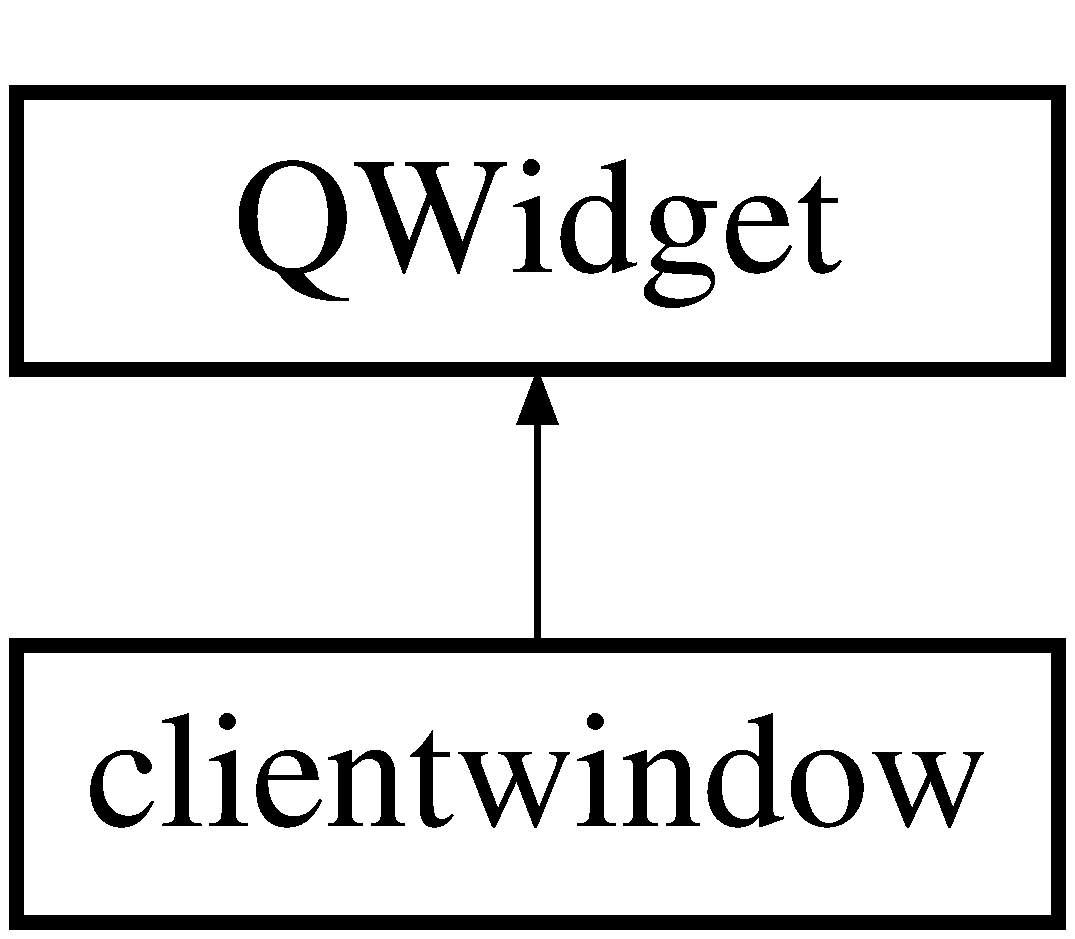
\includegraphics[height=2.000000cm]{classclientwindow}
\end{center}
\end{figure}
\subsection*{Public Slots}
\begin{DoxyCompactItemize}
\item 
void \mbox{\hyperlink{classclientwindow_a0b2358b8e187213e045381ed2d582e3e}{ready\+Read}} ()
\begin{DoxyCompactList}\small\item\em Slot stores all received data from client to received\+Data. \end{DoxyCompactList}\end{DoxyCompactItemize}
\subsection*{Signals}
\begin{DoxyCompactItemize}
\item 
\mbox{\Hypertarget{classclientwindow_a9770acc31c02f795535190e795e616da}\label{classclientwindow_a9770acc31c02f795535190e795e616da}} 
void {\bfseries set\+Active\+Widget} (int active\+Widget)
\end{DoxyCompactItemize}
\subsection*{Public Member Functions}
\begin{DoxyCompactItemize}
\item 
\mbox{\hyperlink{classclientwindow_a9ea65c58093430993fc64bedab0ee6e3}{clientwindow}} (Q\+Widget $\ast$parent=0)
\begin{DoxyCompactList}\small\item\em clientwindow class constructor. \end{DoxyCompactList}\item 
\mbox{\hyperlink{classclientwindow_a53333bf0d133c70836f94ba20242fd36}{$\sim$clientwindow}} ()
\begin{DoxyCompactList}\small\item\em clientwindow class deconstructor \end{DoxyCompactList}\item 
void \mbox{\hyperlink{classclientwindow_af4fa9df47a939b45246e7686d0f8c569}{send\+Data}} (Q\+Byte\+Array string)
\begin{DoxyCompactList}\small\item\em sends data from server\+Socket \end{DoxyCompactList}\item 
Q\+Byte\+Array \mbox{\hyperlink{classclientwindow_aef46aaa18fbaff0c95db9ae6c24a8847}{get\+Received\+Data}} () const
\begin{DoxyCompactList}\small\item\em received\+Data getter. \end{DoxyCompactList}\end{DoxyCompactItemize}


\subsection{Detailed Description}
clientwindow class is responsible for estabilishing connection with server. Class is sending/receiving data over tcp protocol. 

\subsection{Constructor \& Destructor Documentation}
\mbox{\Hypertarget{classclientwindow_a9ea65c58093430993fc64bedab0ee6e3}\label{classclientwindow_a9ea65c58093430993fc64bedab0ee6e3}} 
\index{clientwindow@{clientwindow}!clientwindow@{clientwindow}}
\index{clientwindow@{clientwindow}!clientwindow@{clientwindow}}
\subsubsection{\texorpdfstring{clientwindow()}{clientwindow()}}
{\footnotesize\ttfamily clientwindow\+::clientwindow (\begin{DoxyParamCaption}\item[{Q\+Widget $\ast$}]{parent = {\ttfamily 0} }\end{DoxyParamCaption})\hspace{0.3cm}{\ttfamily [explicit]}}



clientwindow class constructor. 

Creates new tcp client. 
\begin{DoxyParams}{Parameters}
{\em Q\+Widget} & $\ast$parent \\
\hline
\end{DoxyParams}

\begin{DoxyRetVals}{Return values}
{\em void} & \\
\hline
\end{DoxyRetVals}
\mbox{\Hypertarget{classclientwindow_a53333bf0d133c70836f94ba20242fd36}\label{classclientwindow_a53333bf0d133c70836f94ba20242fd36}} 
\index{clientwindow@{clientwindow}!````~clientwindow@{$\sim$clientwindow}}
\index{````~clientwindow@{$\sim$clientwindow}!clientwindow@{clientwindow}}
\subsubsection{\texorpdfstring{$\sim$clientwindow()}{~clientwindow()}}
{\footnotesize\ttfamily clientwindow\+::$\sim$clientwindow (\begin{DoxyParamCaption}{ }\end{DoxyParamCaption})}



clientwindow class deconstructor 


\begin{DoxyParams}{Parameters}
{\em void} & \\
\hline
\end{DoxyParams}
\begin{DoxyReturn}{Returns}
void 
\end{DoxyReturn}


\subsection{Member Function Documentation}
\mbox{\Hypertarget{classclientwindow_aef46aaa18fbaff0c95db9ae6c24a8847}\label{classclientwindow_aef46aaa18fbaff0c95db9ae6c24a8847}} 
\index{clientwindow@{clientwindow}!get\+Received\+Data@{get\+Received\+Data}}
\index{get\+Received\+Data@{get\+Received\+Data}!clientwindow@{clientwindow}}
\subsubsection{\texorpdfstring{get\+Received\+Data()}{getReceivedData()}}
{\footnotesize\ttfamily Q\+Byte\+Array clientwindow\+::get\+Received\+Data (\begin{DoxyParamCaption}{ }\end{DoxyParamCaption}) const}



received\+Data getter. 


\begin{DoxyParams}{Parameters}
{\em void} & \\
\hline
\end{DoxyParams}
\begin{DoxyReturn}{Returns}
Q\+Byte\+Array received\+Data 
\end{DoxyReturn}
\mbox{\Hypertarget{classclientwindow_a0b2358b8e187213e045381ed2d582e3e}\label{classclientwindow_a0b2358b8e187213e045381ed2d582e3e}} 
\index{clientwindow@{clientwindow}!ready\+Read@{ready\+Read}}
\index{ready\+Read@{ready\+Read}!clientwindow@{clientwindow}}
\subsubsection{\texorpdfstring{ready\+Read}{readyRead}}
{\footnotesize\ttfamily void clientwindow\+::ready\+Read (\begin{DoxyParamCaption}{ }\end{DoxyParamCaption})\hspace{0.3cm}{\ttfamily [slot]}}



Slot stores all received data from client to received\+Data. 


\begin{DoxyParams}{Parameters}
{\em void} & \\
\hline
\end{DoxyParams}
\begin{DoxyReturn}{Returns}
void 
\end{DoxyReturn}
\mbox{\Hypertarget{classclientwindow_af4fa9df47a939b45246e7686d0f8c569}\label{classclientwindow_af4fa9df47a939b45246e7686d0f8c569}} 
\index{clientwindow@{clientwindow}!send\+Data@{send\+Data}}
\index{send\+Data@{send\+Data}!clientwindow@{clientwindow}}
\subsubsection{\texorpdfstring{send\+Data()}{sendData()}}
{\footnotesize\ttfamily void clientwindow\+::send\+Data (\begin{DoxyParamCaption}\item[{Q\+Byte\+Array}]{string }\end{DoxyParamCaption})}



sends data from server\+Socket 


\begin{DoxyParams}{Parameters}
{\em Q\+Byte\+Array} & string \\
\hline
\end{DoxyParams}
\begin{DoxyReturn}{Returns}
void 
\end{DoxyReturn}


The documentation for this class was generated from the following files\+:\begin{DoxyCompactItemize}
\item 
clientwindow.\+h\item 
\mbox{\hyperlink{clientwindow_8cpp}{clientwindow.\+cpp}}\end{DoxyCompactItemize}

\hypertarget{classgame_options}{}\section{game\+Options Class Reference}
\label{classgame_options}\index{game\+Options@{game\+Options}}


{\ttfamily \#include $<$gameoptions.\+h$>$}

Inheritance diagram for game\+Options\+:\begin{figure}[H]
\begin{center}
\leavevmode
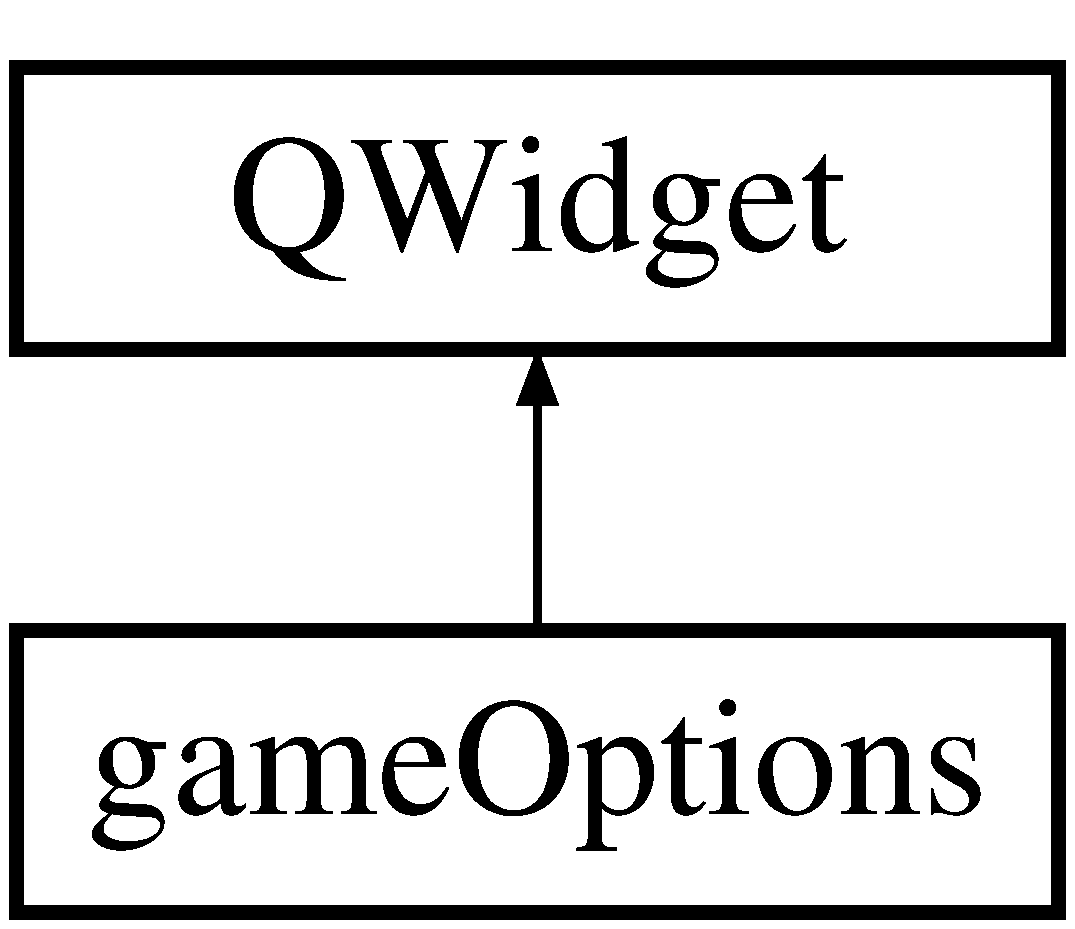
\includegraphics[height=2.000000cm]{classgame_options}
\end{center}
\end{figure}
\subsection*{Signals}
\begin{DoxyCompactItemize}
\item 
\mbox{\Hypertarget{classgame_options_ab3c1e3b2714d32c8c05ebab6392859b5}\label{classgame_options_ab3c1e3b2714d32c8c05ebab6392859b5}} 
void {\bfseries set\+Active\+Widget} (int active\+Widget)
\end{DoxyCompactItemize}
\subsection*{Public Member Functions}
\begin{DoxyCompactItemize}
\item 
\mbox{\hyperlink{classgame_options_a2ebd15d680a6cadd61e9cec3d8968677}{game\+Options}} (Q\+Widget $\ast$parent=0)
\begin{DoxyCompactList}\small\item\em \mbox{\hyperlink{classgame_options}{game\+Options}} class constructor. \end{DoxyCompactList}\item 
\mbox{\hyperlink{classgame_options_ae0f5375ed0aa7e83890ae42ee4b512c3}{$\sim$game\+Options}} ()
\begin{DoxyCompactList}\small\item\em \mbox{\hyperlink{classgame_options}{game\+Options}} class deconstructor. \end{DoxyCompactList}\item 
\mbox{\Hypertarget{classgame_options_a1103c5ad656911a33a12ddd6eee94db8}\label{classgame_options_a1103c5ad656911a33a12ddd6eee94db8}} 
connection\+Role\+Type {\bfseries get\+Connection\+Role} () const
\end{DoxyCompactItemize}


\subsection{Detailed Description}
\mbox{\hyperlink{classgame_options}{game\+Options}} class creates a welcome screen, where user can select to start a game in server or client mode. 

\subsection{Constructor \& Destructor Documentation}
\mbox{\Hypertarget{classgame_options_a2ebd15d680a6cadd61e9cec3d8968677}\label{classgame_options_a2ebd15d680a6cadd61e9cec3d8968677}} 
\index{game\+Options@{game\+Options}!game\+Options@{game\+Options}}
\index{game\+Options@{game\+Options}!game\+Options@{game\+Options}}
\subsubsection{\texorpdfstring{game\+Options()}{gameOptions()}}
{\footnotesize\ttfamily game\+Options\+::game\+Options (\begin{DoxyParamCaption}\item[{Q\+Widget $\ast$}]{parent = {\ttfamily 0} }\end{DoxyParamCaption})\hspace{0.3cm}{\ttfamily [explicit]}}



\mbox{\hyperlink{classgame_options}{game\+Options}} class constructor. 

Sets up windows widget ui. 
\begin{DoxyParams}{Parameters}
{\em Q\+Widget} & $\ast$parent \\
\hline
\end{DoxyParams}
\begin{DoxyReturn}{Returns}
void 
\end{DoxyReturn}
\mbox{\Hypertarget{classgame_options_ae0f5375ed0aa7e83890ae42ee4b512c3}\label{classgame_options_ae0f5375ed0aa7e83890ae42ee4b512c3}} 
\index{game\+Options@{game\+Options}!````~game\+Options@{$\sim$game\+Options}}
\index{````~game\+Options@{$\sim$game\+Options}!game\+Options@{game\+Options}}
\subsubsection{\texorpdfstring{$\sim$game\+Options()}{~gameOptions()}}
{\footnotesize\ttfamily game\+Options\+::$\sim$game\+Options (\begin{DoxyParamCaption}{ }\end{DoxyParamCaption})}



\mbox{\hyperlink{classgame_options}{game\+Options}} class deconstructor. 


\begin{DoxyParams}{Parameters}
{\em void} & \\
\hline
\end{DoxyParams}
\begin{DoxyReturn}{Returns}
void 
\end{DoxyReturn}


The documentation for this class was generated from the following files\+:\begin{DoxyCompactItemize}
\item 
gameoptions.\+h\item 
\mbox{\hyperlink{gameoptions_8cpp}{gameoptions.\+cpp}}\end{DoxyCompactItemize}

\hypertarget{classgame_window}{}\section{game\+Window Class Reference}
\label{classgame_window}\index{game\+Window@{game\+Window}}


{\ttfamily \#include $<$gamewindow.\+h$>$}

Inheritance diagram for game\+Window\+:\begin{figure}[H]
\begin{center}
\leavevmode
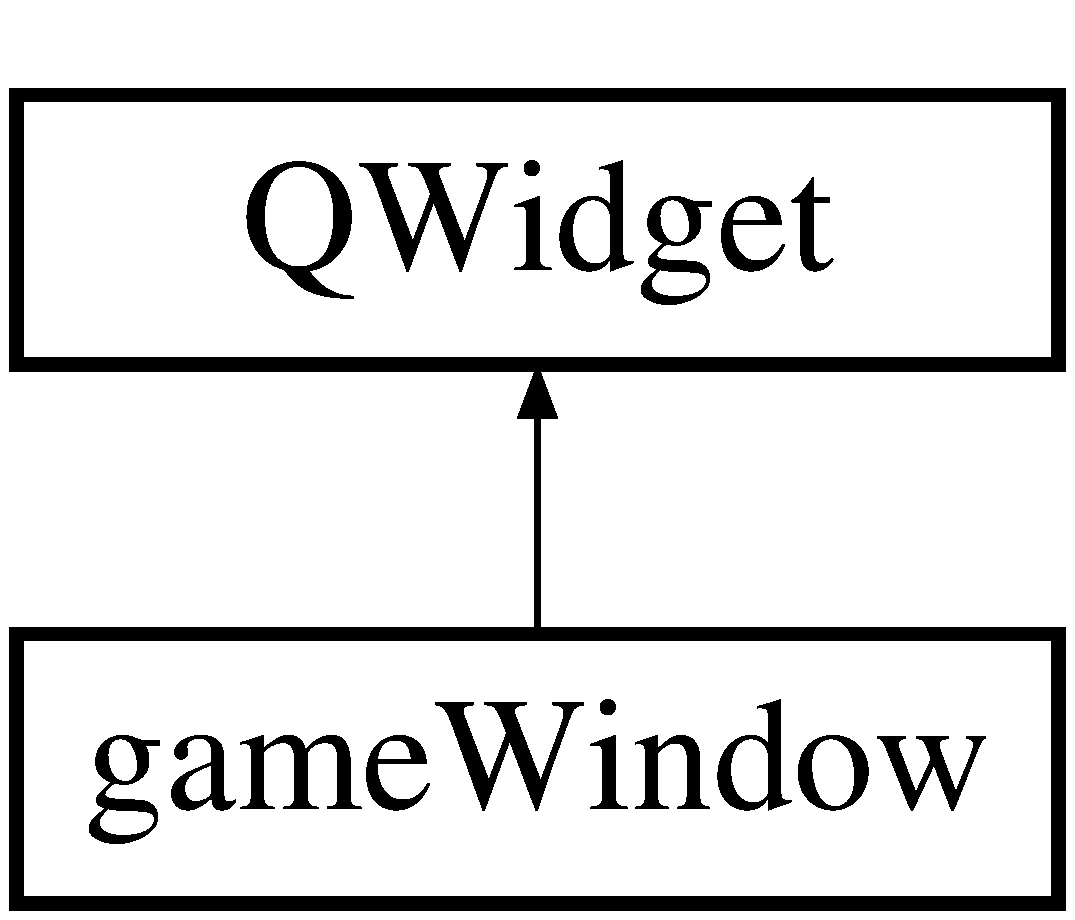
\includegraphics[height=2.000000cm]{classgame_window}
\end{center}
\end{figure}
\subsection*{Public Slots}
\begin{DoxyCompactItemize}
\item 
void \mbox{\hyperlink{classgame_window_a2aeb402950ac1faa754288a9e7464563}{game\+Loop}} (void)
\begin{DoxyCompactList}\small\item\em Game loop -\/ updates game states and variables. \end{DoxyCompactList}\end{DoxyCompactItemize}
\subsection*{Public Member Functions}
\begin{DoxyCompactItemize}
\item 
\mbox{\hyperlink{classgame_window_af31e4cb1c92ed36e03ef264c8d4efa51}{game\+Window}} (Q\+Widget $\ast$parent=0)
\begin{DoxyCompactList}\small\item\em \mbox{\hyperlink{classgame_window}{game\+Window}} class constructor. \end{DoxyCompactList}\item 
\mbox{\hyperlink{classgame_window_a13773b6a92bc1d9a7e0067ed99fa4e20}{$\sim$game\+Window}} ()
\begin{DoxyCompactList}\small\item\em \mbox{\hyperlink{classgame_window}{game\+Window}} class deconstructor \end{DoxyCompactList}\item 
void \mbox{\hyperlink{classgame_window_a790233fd0316f05a1fd35738d383349b}{start\+Game}} (void)
\begin{DoxyCompactList}\small\item\em Start game timer. \end{DoxyCompactList}\item 
\mbox{\Hypertarget{classgame_window_a53a82990ddc2c819e3570ad52b340a90}\label{classgame_window_a53a82990ddc2c819e3570ad52b340a90}} 
\mbox{\hyperlink{classserver_window}{server\+Window}} $\ast$ \mbox{\hyperlink{classgame_window_a53a82990ddc2c819e3570ad52b340a90}{get\+Game\+Server}} () const
\begin{DoxyCompactList}\small\item\em game\+Server getter. \end{DoxyCompactList}\item 
\mbox{\Hypertarget{classgame_window_a488fb57d2d073817325f8128dee0f85d}\label{classgame_window_a488fb57d2d073817325f8128dee0f85d}} 
void \mbox{\hyperlink{classgame_window_a488fb57d2d073817325f8128dee0f85d}{set\+Game\+Server}} (\mbox{\hyperlink{classserver_window}{server\+Window}} $\ast$value)
\begin{DoxyCompactList}\small\item\em game\+Server setter. \end{DoxyCompactList}\item 
\mbox{\Hypertarget{classgame_window_a69e38c52ddea9d76beea2b7ad38b399e}\label{classgame_window_a69e38c52ddea9d76beea2b7ad38b399e}} 
\mbox{\hyperlink{classclientwindow}{clientwindow}} $\ast$ \mbox{\hyperlink{classgame_window_a69e38c52ddea9d76beea2b7ad38b399e}{get\+Game\+Client}} () const
\begin{DoxyCompactList}\small\item\em game\+Client getter. \end{DoxyCompactList}\item 
\mbox{\Hypertarget{classgame_window_ad9fdccffaca852e5f7ad31ec54c0c619}\label{classgame_window_ad9fdccffaca852e5f7ad31ec54c0c619}} 
void \mbox{\hyperlink{classgame_window_ad9fdccffaca852e5f7ad31ec54c0c619}{set\+Game\+Client}} (\mbox{\hyperlink{classclientwindow}{clientwindow}} $\ast$value)
\begin{DoxyCompactList}\small\item\em game\+Client setter. \end{DoxyCompactList}\item 
\mbox{\Hypertarget{classgame_window_ad597375ea2f848cf27da3eb725219c53}\label{classgame_window_ad597375ea2f848cf27da3eb725219c53}} 
connection\+Role\+Type \mbox{\hyperlink{classgame_window_ad597375ea2f848cf27da3eb725219c53}{get\+Connection\+Role}} () const
\begin{DoxyCompactList}\small\item\em connection\+Role getter. \end{DoxyCompactList}\item 
\mbox{\Hypertarget{classgame_window_ad00607412c93c7b157ef7e3ec1a2e7df}\label{classgame_window_ad00607412c93c7b157ef7e3ec1a2e7df}} 
void \mbox{\hyperlink{classgame_window_ad00607412c93c7b157ef7e3ec1a2e7df}{set\+Connection\+Role}} (const connection\+Role\+Type \&value)
\begin{DoxyCompactList}\small\item\em connection\+Role setter. \end{DoxyCompactList}\end{DoxyCompactItemize}
\subsection*{Protected Attributes}
\begin{DoxyCompactItemize}
\item 
\mbox{\Hypertarget{classgame_window_a22f5b5b08120edb4eb1e15845efd07ec}\label{classgame_window_a22f5b5b08120edb4eb1e15845efd07ec}} 
Q\+Graphics\+Scene $\ast$ \mbox{\hyperlink{classgame_window_a22f5b5b08120edb4eb1e15845efd07ec}{scene}}
\begin{DoxyCompactList}\small\item\em Game images are drawn on this scene. \end{DoxyCompactList}\end{DoxyCompactItemize}


\subsection{Detailed Description}
\mbox{\hyperlink{classgame_window}{game\+Window}} controlls game logic, creates all actors and maintains connection and data flow between server and client. 

\subsection{Constructor \& Destructor Documentation}
\mbox{\Hypertarget{classgame_window_af31e4cb1c92ed36e03ef264c8d4efa51}\label{classgame_window_af31e4cb1c92ed36e03ef264c8d4efa51}} 
\index{game\+Window@{game\+Window}!game\+Window@{game\+Window}}
\index{game\+Window@{game\+Window}!game\+Window@{game\+Window}}
\subsubsection{\texorpdfstring{game\+Window()}{gameWindow()}}
{\footnotesize\ttfamily game\+Window\+::game\+Window (\begin{DoxyParamCaption}\item[{Q\+Widget $\ast$}]{parent = {\ttfamily 0} }\end{DoxyParamCaption})\hspace{0.3cm}{\ttfamily [explicit]}}



\mbox{\hyperlink{classgame_window}{game\+Window}} class constructor. 

Constructor initializs graphics elements of game board, initializes map tiles and adds actors to the board. 
\begin{DoxyParams}{Parameters}
{\em Q\+Widget} & $\ast$parent \\
\hline
\end{DoxyParams}

\begin{DoxyRetVals}{Return values}
{\em void} & \\
\hline
\end{DoxyRetVals}
\mbox{\Hypertarget{classgame_window_a13773b6a92bc1d9a7e0067ed99fa4e20}\label{classgame_window_a13773b6a92bc1d9a7e0067ed99fa4e20}} 
\index{game\+Window@{game\+Window}!````~game\+Window@{$\sim$game\+Window}}
\index{````~game\+Window@{$\sim$game\+Window}!game\+Window@{game\+Window}}
\subsubsection{\texorpdfstring{$\sim$game\+Window()}{~gameWindow()}}
{\footnotesize\ttfamily game\+Window\+::$\sim$game\+Window (\begin{DoxyParamCaption}{ }\end{DoxyParamCaption})}



\mbox{\hyperlink{classgame_window}{game\+Window}} class deconstructor 


\begin{DoxyParams}{Parameters}
{\em void} & \\
\hline
\end{DoxyParams}
\begin{DoxyReturn}{Returns}
void 
\end{DoxyReturn}


\subsection{Member Function Documentation}
\mbox{\Hypertarget{classgame_window_a2aeb402950ac1faa754288a9e7464563}\label{classgame_window_a2aeb402950ac1faa754288a9e7464563}} 
\index{game\+Window@{game\+Window}!game\+Loop@{game\+Loop}}
\index{game\+Loop@{game\+Loop}!game\+Window@{game\+Window}}
\subsubsection{\texorpdfstring{game\+Loop}{gameLoop}}
{\footnotesize\ttfamily void game\+Window\+::game\+Loop (\begin{DoxyParamCaption}\item[{void}]{ }\end{DoxyParamCaption})\hspace{0.3cm}{\ttfamily [slot]}}



Game loop -\/ updates game states and variables. 

This function is a slot for Timer. This function is called after each Timer overflow. Game logic is based on connection\+Role. Part of the gameloop is executed on server and part on client side. 
\begin{DoxyParams}{Parameters}
{\em void} & \\
\hline
\end{DoxyParams}
\begin{DoxyReturn}{Returns}
void 
\end{DoxyReturn}
\mbox{\Hypertarget{classgame_window_a790233fd0316f05a1fd35738d383349b}\label{classgame_window_a790233fd0316f05a1fd35738d383349b}} 
\index{game\+Window@{game\+Window}!start\+Game@{start\+Game}}
\index{start\+Game@{start\+Game}!game\+Window@{game\+Window}}
\subsubsection{\texorpdfstring{start\+Game()}{startGame()}}
{\footnotesize\ttfamily void game\+Window\+::start\+Game (\begin{DoxyParamCaption}\item[{void}]{ }\end{DoxyParamCaption})}



Start game timer. 


\begin{DoxyParams}{Parameters}
{\em void} & \\
\hline
\end{DoxyParams}
\begin{DoxyReturn}{Returns}
void 
\end{DoxyReturn}


The documentation for this class was generated from the following files\+:\begin{DoxyCompactItemize}
\item 
gamewindow.\+h\item 
\mbox{\hyperlink{gamewindow_8cpp}{gamewindow.\+cpp}}\end{DoxyCompactItemize}

\hypertarget{class_ghost}{}\section{Ghost Class Reference}
\label{class_ghost}\index{Ghost@{Ghost}}


{\ttfamily \#include $<$ghost.\+h$>$}

Inheritance diagram for Ghost\+:\begin{figure}[H]
\begin{center}
\leavevmode
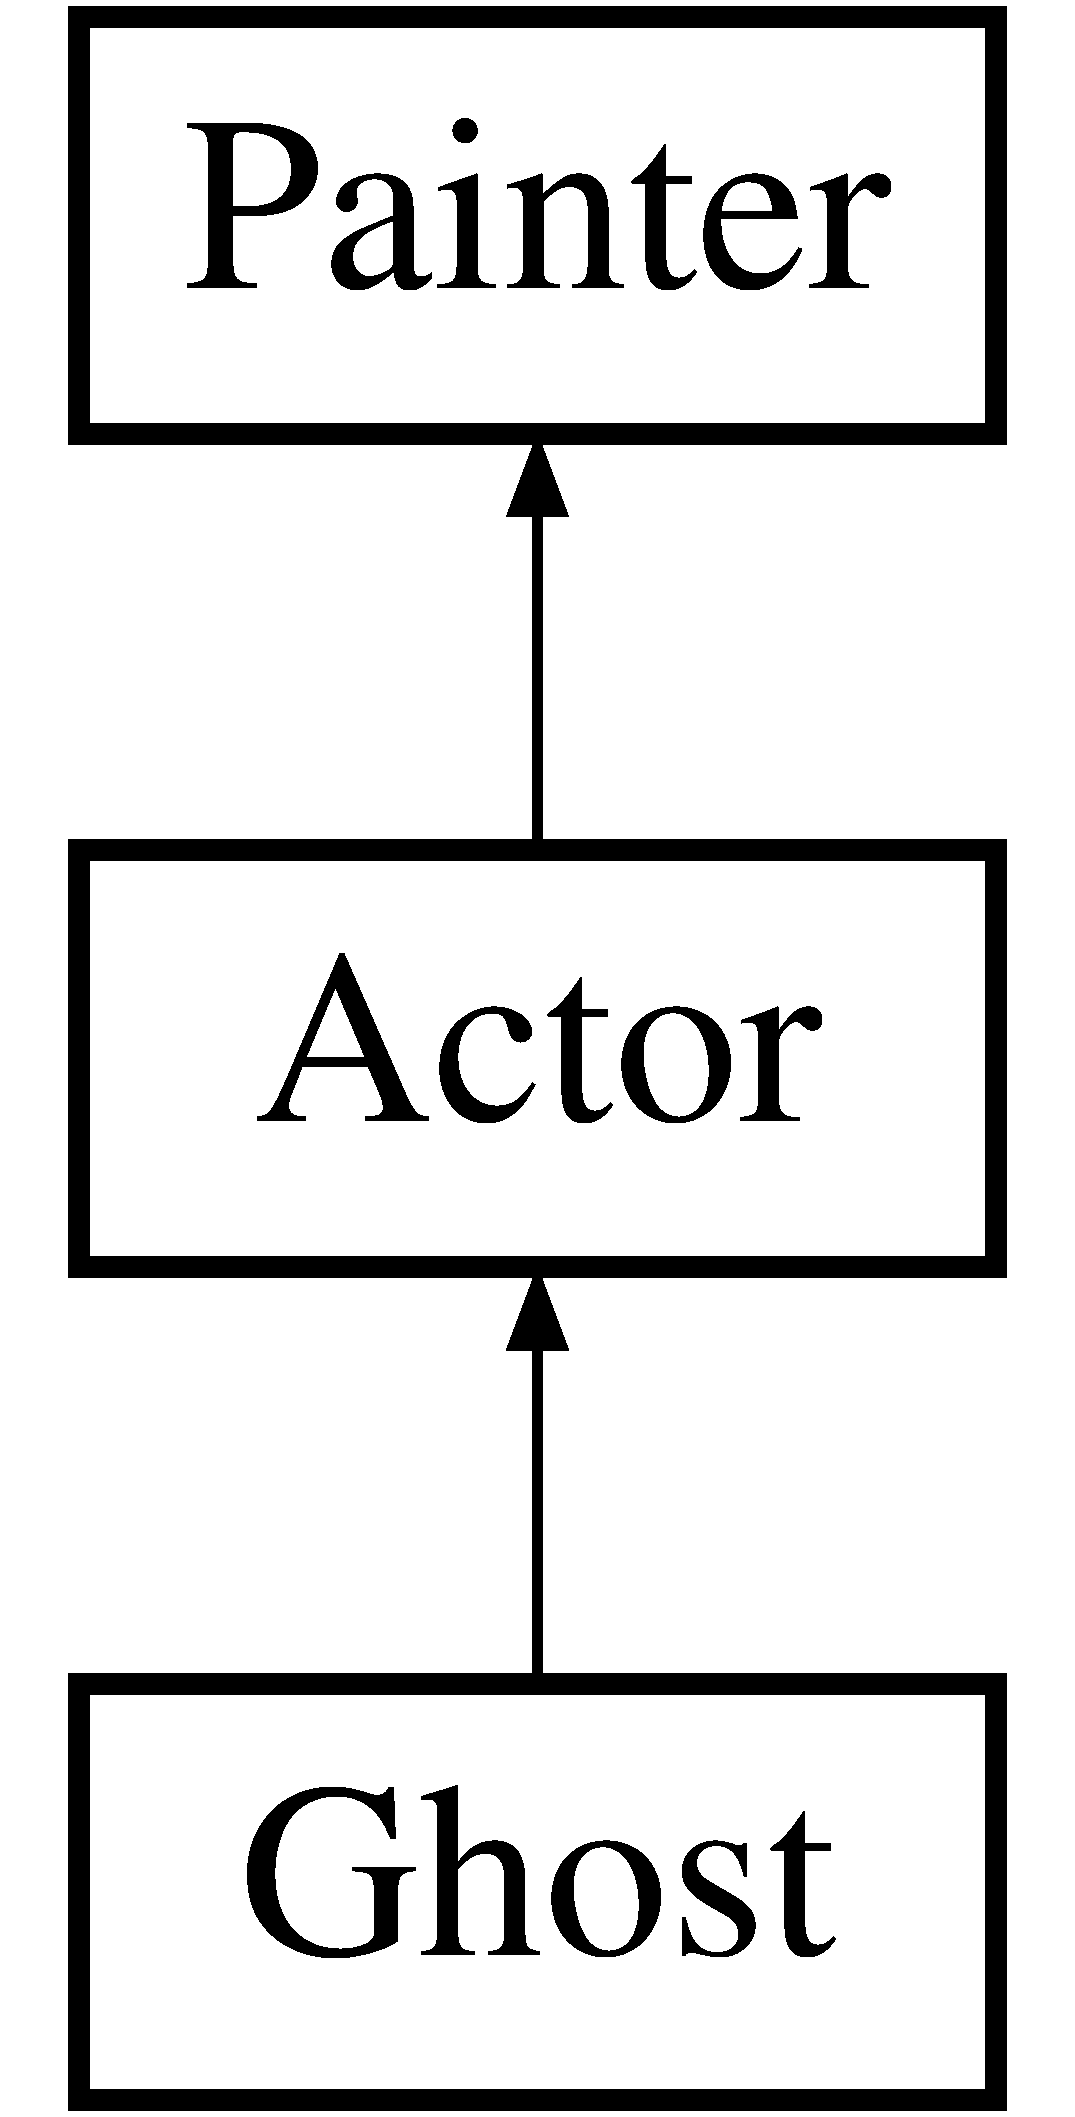
\includegraphics[height=3.000000cm]{class_ghost}
\end{center}
\end{figure}
\subsection*{Public Member Functions}
\begin{DoxyCompactItemize}
\item 
\mbox{\hyperlink{class_ghost_a2e38d3c0c8546cceb74777b49a8e3bb7}{Ghost}} ()
\begin{DoxyCompactList}\small\item\em Empty \mbox{\hyperlink{class_ghost}{Ghost}} class constructor. \end{DoxyCompactList}\item 
\mbox{\hyperlink{class_ghost_a3b8caf4d2c5a166c05f29e8478abdb4c}{Ghost}} (Q\+String pixmap\+Path, int x, int y)
\begin{DoxyCompactList}\small\item\em Overloaded \mbox{\hyperlink{class_ghost}{Ghost}} class constructor. \end{DoxyCompactList}\end{DoxyCompactItemize}
\subsection*{Additional Inherited Members}


\subsection{Detailed Description}
\mbox{\hyperlink{class_ghost}{Ghost}} class inherits \mbox{\hyperlink{class_actor}{Actor}} class. Class is responsible for controlling Ghosts. 

\subsection{Constructor \& Destructor Documentation}
\mbox{\Hypertarget{class_ghost_a2e38d3c0c8546cceb74777b49a8e3bb7}\label{class_ghost_a2e38d3c0c8546cceb74777b49a8e3bb7}} 
\index{Ghost@{Ghost}!Ghost@{Ghost}}
\index{Ghost@{Ghost}!Ghost@{Ghost}}
\subsubsection{\texorpdfstring{Ghost()}{Ghost()}\hspace{0.1cm}{\footnotesize\ttfamily [1/2]}}
{\footnotesize\ttfamily Ghost\+::\+Ghost (\begin{DoxyParamCaption}{ }\end{DoxyParamCaption})}



Empty \mbox{\hyperlink{class_ghost}{Ghost}} class constructor. 


\begin{DoxyParams}{Parameters}
{\em void} & \\
\hline
\end{DoxyParams}
\begin{DoxyReturn}{Returns}
void 
\end{DoxyReturn}
\mbox{\Hypertarget{class_ghost_a3b8caf4d2c5a166c05f29e8478abdb4c}\label{class_ghost_a3b8caf4d2c5a166c05f29e8478abdb4c}} 
\index{Ghost@{Ghost}!Ghost@{Ghost}}
\index{Ghost@{Ghost}!Ghost@{Ghost}}
\subsubsection{\texorpdfstring{Ghost()}{Ghost()}\hspace{0.1cm}{\footnotesize\ttfamily [2/2]}}
{\footnotesize\ttfamily Ghost\+::\+Ghost (\begin{DoxyParamCaption}\item[{Q\+String}]{pixmap\+Path,  }\item[{int}]{x,  }\item[{int}]{y }\end{DoxyParamCaption})}



Overloaded \mbox{\hyperlink{class_ghost}{Ghost}} class constructor. 

Updates \mbox{\hyperlink{class_ghost}{Ghost}} graphics, sets x and y positions. 
\begin{DoxyParams}{Parameters}
{\em Q\+String} & pixmap\+Path, int x, int y \\
\hline
\end{DoxyParams}
\begin{DoxyReturn}{Returns}
void 
\end{DoxyReturn}


The documentation for this class was generated from the following files\+:\begin{DoxyCompactItemize}
\item 
ghost.\+h\item 
\mbox{\hyperlink{ghost_8cpp}{ghost.\+cpp}}\end{DoxyCompactItemize}

\hypertarget{class_main_window}{}\section{Main\+Window Class Reference}
\label{class_main_window}\index{Main\+Window@{Main\+Window}}


{\ttfamily \#include $<$mainwindow.\+h$>$}

Inheritance diagram for Main\+Window\+:\begin{figure}[H]
\begin{center}
\leavevmode
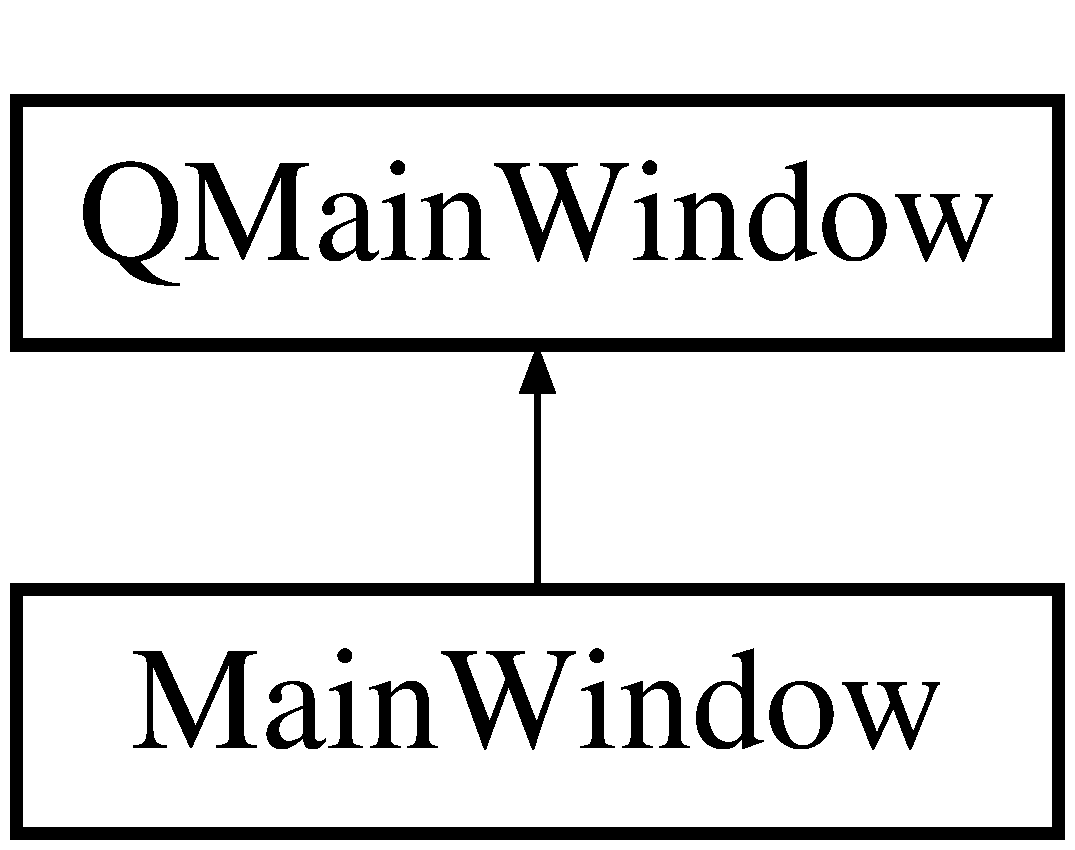
\includegraphics[height=2.000000cm]{class_main_window}
\end{center}
\end{figure}
\subsection*{Public Member Functions}
\begin{DoxyCompactItemize}
\item 
\mbox{\hyperlink{class_main_window_a8b244be8b7b7db1b08de2a2acb9409db}{Main\+Window}} (Q\+Widget $\ast$parent=0)
\begin{DoxyCompactList}\small\item\em \mbox{\hyperlink{class_main_window}{Main\+Window}} class constructor. \end{DoxyCompactList}\item 
\mbox{\hyperlink{class_main_window_ae98d00a93bc118200eeef9f9bba1dba7}{$\sim$\+Main\+Window}} ()
\begin{DoxyCompactList}\small\item\em \mbox{\hyperlink{class_main_window}{Main\+Window}} class deconstructor. \end{DoxyCompactList}\end{DoxyCompactItemize}


\subsection{Detailed Description}
\mbox{\hyperlink{class_main_window}{Main\+Window}} class is responsible for switching between active windows. 

\subsection{Constructor \& Destructor Documentation}
\mbox{\Hypertarget{class_main_window_a8b244be8b7b7db1b08de2a2acb9409db}\label{class_main_window_a8b244be8b7b7db1b08de2a2acb9409db}} 
\index{Main\+Window@{Main\+Window}!Main\+Window@{Main\+Window}}
\index{Main\+Window@{Main\+Window}!Main\+Window@{Main\+Window}}
\subsubsection{\texorpdfstring{Main\+Window()}{MainWindow()}}
{\footnotesize\ttfamily Main\+Window\+::\+Main\+Window (\begin{DoxyParamCaption}\item[{Q\+Widget $\ast$}]{parent = {\ttfamily 0} }\end{DoxyParamCaption})\hspace{0.3cm}{\ttfamily [explicit]}}



\mbox{\hyperlink{class_main_window}{Main\+Window}} class constructor. 

Initializes all game widget windows, setsup stacked\+Widget view. 
\begin{DoxyParams}{Parameters}
{\em Q\+Widget} & $\ast$parent \\
\hline
\end{DoxyParams}

\begin{DoxyRetVals}{Return values}
{\em void} & \\
\hline
\end{DoxyRetVals}
\mbox{\Hypertarget{class_main_window_ae98d00a93bc118200eeef9f9bba1dba7}\label{class_main_window_ae98d00a93bc118200eeef9f9bba1dba7}} 
\index{Main\+Window@{Main\+Window}!````~Main\+Window@{$\sim$\+Main\+Window}}
\index{````~Main\+Window@{$\sim$\+Main\+Window}!Main\+Window@{Main\+Window}}
\subsubsection{\texorpdfstring{$\sim$\+Main\+Window()}{~MainWindow()}}
{\footnotesize\ttfamily Main\+Window\+::$\sim$\+Main\+Window (\begin{DoxyParamCaption}{ }\end{DoxyParamCaption})}



\mbox{\hyperlink{class_main_window}{Main\+Window}} class deconstructor. 


\begin{DoxyParams}{Parameters}
{\em void} & \\
\hline
\end{DoxyParams}
\begin{DoxyReturn}{Returns}
void 
\end{DoxyReturn}


The documentation for this class was generated from the following files\+:\begin{DoxyCompactItemize}
\item 
mainwindow.\+h\item 
\mbox{\hyperlink{mainwindow_8cpp}{mainwindow.\+cpp}}\end{DoxyCompactItemize}

\hypertarget{class_pacman}{}\section{Pacman Class Reference}
\label{class_pacman}\index{Pacman@{Pacman}}


{\ttfamily \#include $<$pacman.\+h$>$}

Inheritance diagram for Pacman\+:\begin{figure}[H]
\begin{center}
\leavevmode
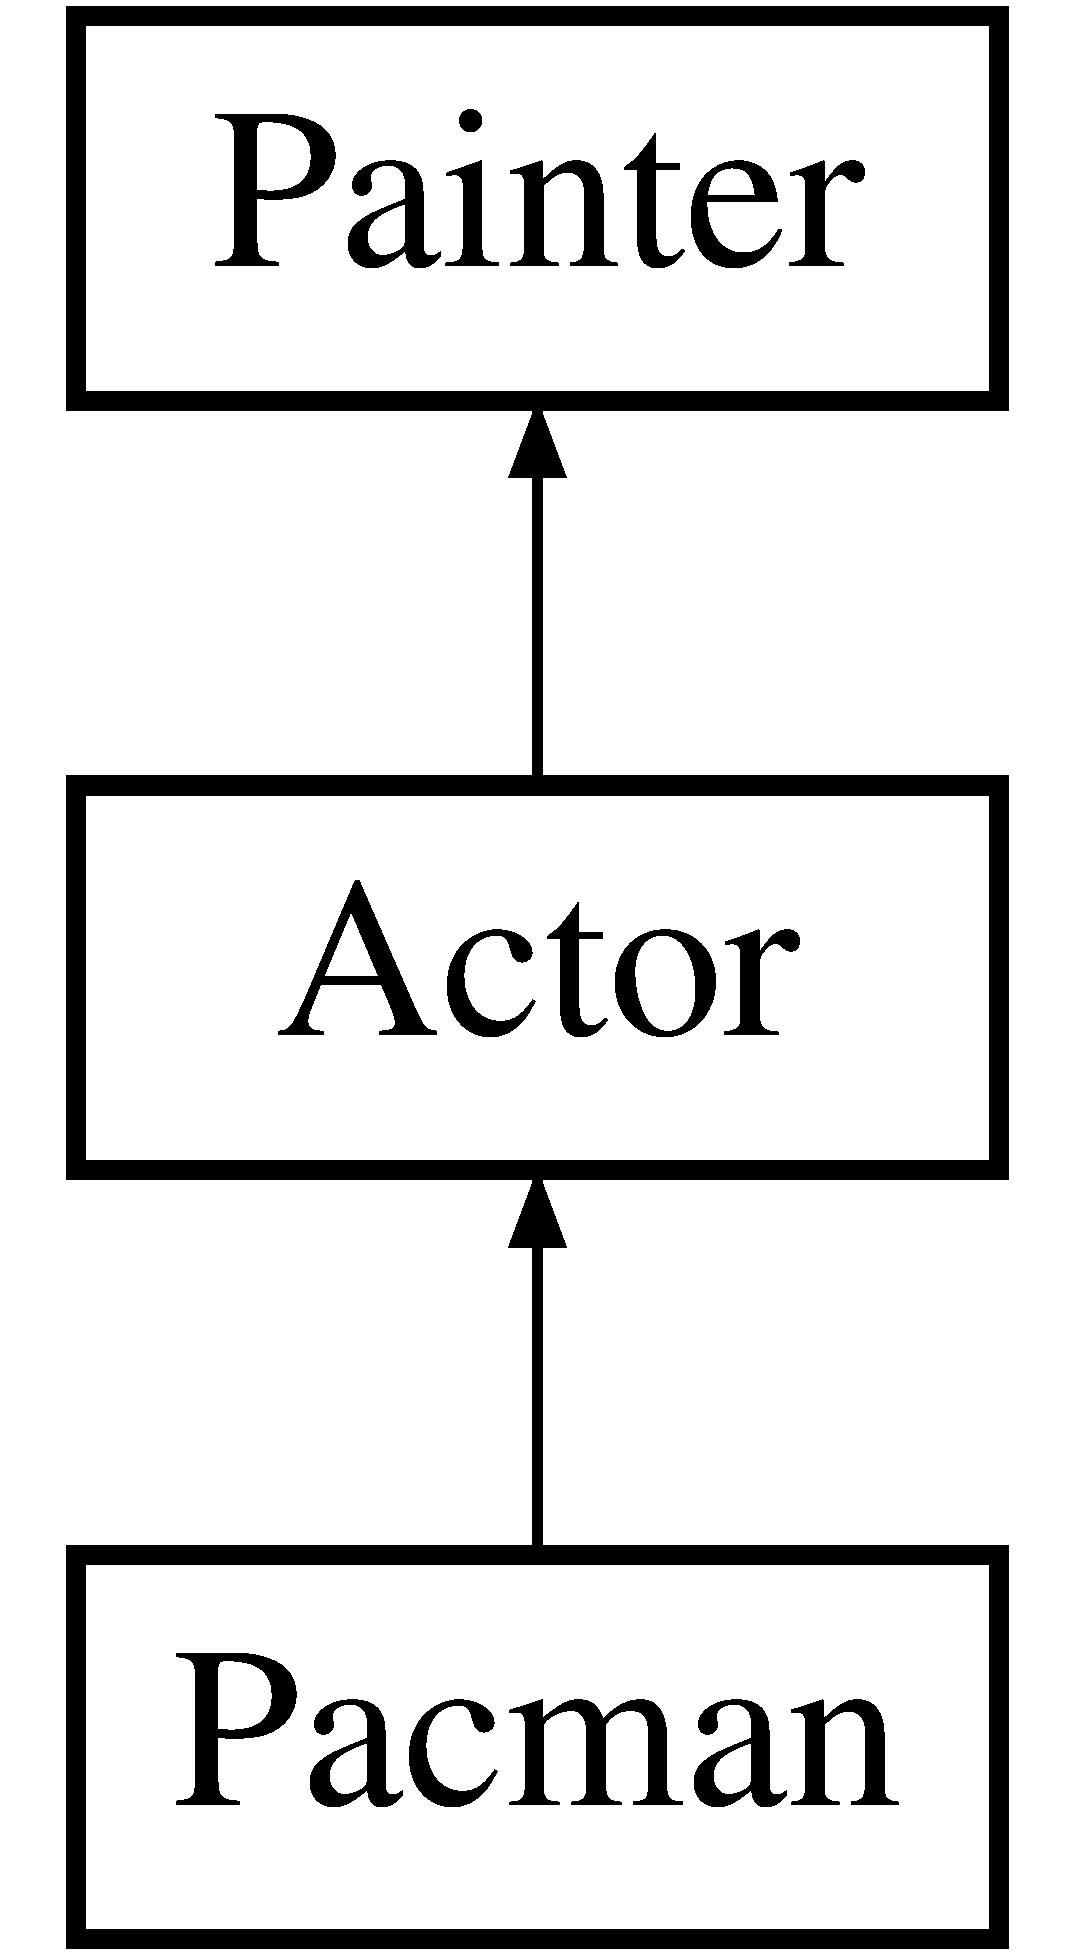
\includegraphics[height=3.000000cm]{class_pacman}
\end{center}
\end{figure}
\subsection*{Public Member Functions}
\begin{DoxyCompactItemize}
\item 
\mbox{\hyperlink{class_pacman_a499408baab38f119ebd4f41e90fbe3fe}{Pacman}} ()
\begin{DoxyCompactList}\small\item\em Empty actor class constructor. \end{DoxyCompactList}\item 
\mbox{\hyperlink{class_pacman_af7a106cbda2c19a855f87dcbac2bfcf5}{Pacman}} (Q\+String pixmap\+Path, int x, int y)
\begin{DoxyCompactList}\small\item\em Overloaded actor class constructor. \end{DoxyCompactList}\item 
\mbox{\Hypertarget{class_pacman_a1a5ec305e9c5951128843ef1035aca2d}\label{class_pacman_a1a5ec305e9c5951128843ef1035aca2d}} 
int \mbox{\hyperlink{class_pacman_a1a5ec305e9c5951128843ef1035aca2d}{get\+Num\+Of\+Lifes}} () const
\begin{DoxyCompactList}\small\item\em num\+Of\+Lifes getter. \end{DoxyCompactList}\item 
\mbox{\Hypertarget{class_pacman_a648f2e202abf2b944d1981865a957ed9}\label{class_pacman_a648f2e202abf2b944d1981865a957ed9}} 
void \mbox{\hyperlink{class_pacman_a648f2e202abf2b944d1981865a957ed9}{set\+Num\+Of\+Lifes}} (int value)
\begin{DoxyCompactList}\small\item\em num\+Of\+Lifes setter. \end{DoxyCompactList}\item 
\mbox{\Hypertarget{class_pacman_aef66596227d1291f5b98141b707fa84c}\label{class_pacman_aef66596227d1291f5b98141b707fa84c}} 
int \mbox{\hyperlink{class_pacman_aef66596227d1291f5b98141b707fa84c}{get\+Points}} () const
\begin{DoxyCompactList}\small\item\em points getter. \end{DoxyCompactList}\item 
\mbox{\Hypertarget{class_pacman_a33eb0d7039987984eaf35ce623af9d83}\label{class_pacman_a33eb0d7039987984eaf35ce623af9d83}} 
void \mbox{\hyperlink{class_pacman_a33eb0d7039987984eaf35ce623af9d83}{set\+Points}} (int value)
\begin{DoxyCompactList}\small\item\em points setter. \end{DoxyCompactList}\end{DoxyCompactItemize}
\subsection*{Additional Inherited Members}


\subsection{Detailed Description}
\mbox{\hyperlink{class_pacman}{Pacman}} class inherits \mbox{\hyperlink{class_actor}{Actor}} class. Class is responsible for controlling Ghosts. 

\subsection{Constructor \& Destructor Documentation}
\mbox{\Hypertarget{class_pacman_a499408baab38f119ebd4f41e90fbe3fe}\label{class_pacman_a499408baab38f119ebd4f41e90fbe3fe}} 
\index{Pacman@{Pacman}!Pacman@{Pacman}}
\index{Pacman@{Pacman}!Pacman@{Pacman}}
\subsubsection{\texorpdfstring{Pacman()}{Pacman()}\hspace{0.1cm}{\footnotesize\ttfamily [1/2]}}
{\footnotesize\ttfamily Pacman\+::\+Pacman (\begin{DoxyParamCaption}{ }\end{DoxyParamCaption})}



Empty actor class constructor. 


\begin{DoxyParams}{Parameters}
{\em void} & \\
\hline
\end{DoxyParams}
\begin{DoxyReturn}{Returns}
void 
\end{DoxyReturn}
\mbox{\Hypertarget{class_pacman_af7a106cbda2c19a855f87dcbac2bfcf5}\label{class_pacman_af7a106cbda2c19a855f87dcbac2bfcf5}} 
\index{Pacman@{Pacman}!Pacman@{Pacman}}
\index{Pacman@{Pacman}!Pacman@{Pacman}}
\subsubsection{\texorpdfstring{Pacman()}{Pacman()}\hspace{0.1cm}{\footnotesize\ttfamily [2/2]}}
{\footnotesize\ttfamily Pacman\+::\+Pacman (\begin{DoxyParamCaption}\item[{Q\+String}]{pixmap\+Path,  }\item[{int}]{x,  }\item[{int}]{y }\end{DoxyParamCaption})}



Overloaded actor class constructor. 

Updates \mbox{\hyperlink{class_pacman}{Pacman}} graphics, sets x and y positions, sets initial number of lives and points. 
\begin{DoxyParams}{Parameters}
{\em Q\+String} & pixmap\+Path, int x, int y \\
\hline
\end{DoxyParams}
\begin{DoxyReturn}{Returns}
void 
\end{DoxyReturn}


The documentation for this class was generated from the following files\+:\begin{DoxyCompactItemize}
\item 
pacman.\+h\item 
\mbox{\hyperlink{pacman_8cpp}{pacman.\+cpp}}\end{DoxyCompactItemize}

\hypertarget{class_painter}{}\section{Painter Class Reference}
\label{class_painter}\index{Painter@{Painter}}


{\ttfamily \#include $<$painter.\+h$>$}

Inheritance diagram for Painter\+:\begin{figure}[H]
\begin{center}
\leavevmode
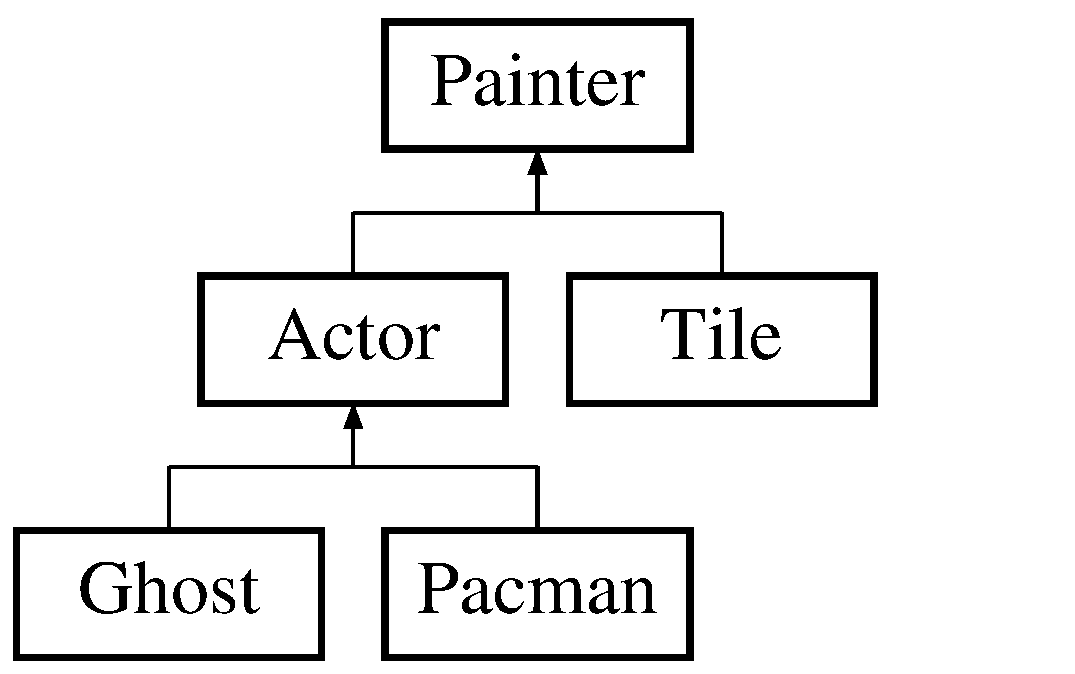
\includegraphics[height=3.000000cm]{class_painter}
\end{center}
\end{figure}
\subsection*{Public Member Functions}
\begin{DoxyCompactItemize}
\item 
\mbox{\hyperlink{class_painter_a32e59ad4d0e130f57c419bd9e9c84675}{Painter}} ()
\begin{DoxyCompactList}\small\item\em Empty \mbox{\hyperlink{class_painter}{Painter}} class constructor. \end{DoxyCompactList}\item 
\mbox{\hyperlink{class_painter_a8a03ffdfcd500771584e662c1de2ef25}{Painter}} (Q\+String pixmap\+Path, int x, int y)
\begin{DoxyCompactList}\small\item\em Overloaded \mbox{\hyperlink{class_painter}{Painter}} class constructor. \end{DoxyCompactList}\item 
void \mbox{\hyperlink{class_painter_a28975648307f4885c65769088dfc7236}{update\+Pos}} (void)
\begin{DoxyCompactList}\small\item\em Updates graphics. \end{DoxyCompactList}\item 
void \mbox{\hyperlink{class_painter_a37b3c5e56ec8ae79c781a4f022082c5f}{set\+Location}} (int x, int y)
\begin{DoxyCompactList}\small\item\em Sets x and y position. \end{DoxyCompactList}\item 
\mbox{\Hypertarget{class_painter_aee846fac5a2a67d71133a9daed1c24fe}\label{class_painter_aee846fac5a2a67d71133a9daed1c24fe}} 
Q\+Pixmap $\ast$ \mbox{\hyperlink{class_painter_aee846fac5a2a67d71133a9daed1c24fe}{get\+Pixmap}} () const
\begin{DoxyCompactList}\small\item\em pixmap getter. \end{DoxyCompactList}\item 
\mbox{\Hypertarget{class_painter_a6439d816409cc7fbf3aa751a94e6771f}\label{class_painter_a6439d816409cc7fbf3aa751a94e6771f}} 
void \mbox{\hyperlink{class_painter_a6439d816409cc7fbf3aa751a94e6771f}{set\+Pixmap}} (Q\+String value)
\begin{DoxyCompactList}\small\item\em pixmap setter. \end{DoxyCompactList}\item 
\mbox{\Hypertarget{class_painter_a7a3890c8c871315a3eb88a2e170949b3}\label{class_painter_a7a3890c8c871315a3eb88a2e170949b3}} 
Q\+Graphics\+Pixmap\+Item $\ast$ \mbox{\hyperlink{class_painter_a7a3890c8c871315a3eb88a2e170949b3}{get\+Pixmap\+Item}} () const
\begin{DoxyCompactList}\small\item\em pixmap\+Item getter. \end{DoxyCompactList}\item 
\mbox{\Hypertarget{class_painter_a0c1b4dff1b51f773f145c373d5e9eef9}\label{class_painter_a0c1b4dff1b51f773f145c373d5e9eef9}} 
int \mbox{\hyperlink{class_painter_a0c1b4dff1b51f773f145c373d5e9eef9}{get\+X\+Pos}} () const
\begin{DoxyCompactList}\small\item\em x\+Pos getter. \end{DoxyCompactList}\item 
\mbox{\Hypertarget{class_painter_a6160fe9c0b29ea1d463d25d52b171b98}\label{class_painter_a6160fe9c0b29ea1d463d25d52b171b98}} 
void \mbox{\hyperlink{class_painter_a6160fe9c0b29ea1d463d25d52b171b98}{set\+X\+Pos}} (int value)
\begin{DoxyCompactList}\small\item\em x\+Pos setter. \end{DoxyCompactList}\item 
\mbox{\Hypertarget{class_painter_aaf3dc8e9e8a4cc69a6f06d57e4168269}\label{class_painter_aaf3dc8e9e8a4cc69a6f06d57e4168269}} 
int \mbox{\hyperlink{class_painter_aaf3dc8e9e8a4cc69a6f06d57e4168269}{get\+Y\+Pos}} () const
\begin{DoxyCompactList}\small\item\em y\+Pos getter. \end{DoxyCompactList}\item 
\mbox{\Hypertarget{class_painter_a6707d7f9bd221764a08f4b5ecb859bba}\label{class_painter_a6707d7f9bd221764a08f4b5ecb859bba}} 
void \mbox{\hyperlink{class_painter_a6707d7f9bd221764a08f4b5ecb859bba}{set\+Y\+Pos}} (int value)
\begin{DoxyCompactList}\small\item\em y\+Pos setter. \end{DoxyCompactList}\end{DoxyCompactItemize}
\subsection*{Protected Attributes}
\begin{DoxyCompactItemize}
\item 
\mbox{\Hypertarget{class_painter_a1af64c4dbd97392dce9940712463d188}\label{class_painter_a1af64c4dbd97392dce9940712463d188}} 
Q\+Pixmap $\ast$ \mbox{\hyperlink{class_painter_a1af64c4dbd97392dce9940712463d188}{pixmap}}
\begin{DoxyCompactList}\small\item\em pixmap is storing image. \end{DoxyCompactList}\item 
\mbox{\Hypertarget{class_painter_a1f3af3b5da3bea41c3fcffc1ad0d6166}\label{class_painter_a1f3af3b5da3bea41c3fcffc1ad0d6166}} 
Q\+Graphics\+Pixmap\+Item $\ast$ \mbox{\hyperlink{class_painter_a1f3af3b5da3bea41c3fcffc1ad0d6166}{pixmap\+Item}}
\begin{DoxyCompactList}\small\item\em pixmap is storing image -\/ used on Q\+Graphics\+Scene. \end{DoxyCompactList}\item 
\mbox{\Hypertarget{class_painter_aae86011c3335c3d63da42d557938ce7d}\label{class_painter_aae86011c3335c3d63da42d557938ce7d}} 
int \mbox{\hyperlink{class_painter_aae86011c3335c3d63da42d557938ce7d}{x\+Pos}}
\begin{DoxyCompactList}\small\item\em x position. \end{DoxyCompactList}\item 
\mbox{\Hypertarget{class_painter_ad38c8bd94f3561b4ffb490ad06935ff2}\label{class_painter_ad38c8bd94f3561b4ffb490ad06935ff2}} 
int \mbox{\hyperlink{class_painter_ad38c8bd94f3561b4ffb490ad06935ff2}{y\+Pos}}
\begin{DoxyCompactList}\small\item\em y position. \end{DoxyCompactList}\end{DoxyCompactItemize}


\subsection{Detailed Description}
\mbox{\hyperlink{class_painter}{Painter}} class is responsible for drawing all images. 

\subsection{Constructor \& Destructor Documentation}
\mbox{\Hypertarget{class_painter_a32e59ad4d0e130f57c419bd9e9c84675}\label{class_painter_a32e59ad4d0e130f57c419bd9e9c84675}} 
\index{Painter@{Painter}!Painter@{Painter}}
\index{Painter@{Painter}!Painter@{Painter}}
\subsubsection{\texorpdfstring{Painter()}{Painter()}\hspace{0.1cm}{\footnotesize\ttfamily [1/2]}}
{\footnotesize\ttfamily Painter\+::\+Painter (\begin{DoxyParamCaption}{ }\end{DoxyParamCaption})}



Empty \mbox{\hyperlink{class_painter}{Painter}} class constructor. 


\begin{DoxyParams}{Parameters}
{\em void} & \\
\hline
\end{DoxyParams}
\begin{DoxyReturn}{Returns}
void 
\end{DoxyReturn}
\mbox{\Hypertarget{class_painter_a8a03ffdfcd500771584e662c1de2ef25}\label{class_painter_a8a03ffdfcd500771584e662c1de2ef25}} 
\index{Painter@{Painter}!Painter@{Painter}}
\index{Painter@{Painter}!Painter@{Painter}}
\subsubsection{\texorpdfstring{Painter()}{Painter()}\hspace{0.1cm}{\footnotesize\ttfamily [2/2]}}
{\footnotesize\ttfamily Painter\+::\+Painter (\begin{DoxyParamCaption}\item[{Q\+String}]{pixmap\+Path,  }\item[{int}]{x,  }\item[{int}]{y }\end{DoxyParamCaption})}



Overloaded \mbox{\hyperlink{class_painter}{Painter}} class constructor. 

Updates graphics, sets x and y positions. 
\begin{DoxyParams}{Parameters}
{\em Q\+String} & pixmap\+Path, int x, int y \\
\hline
\end{DoxyParams}
\begin{DoxyReturn}{Returns}
void 
\end{DoxyReturn}


\subsection{Member Function Documentation}
\mbox{\Hypertarget{class_painter_a37b3c5e56ec8ae79c781a4f022082c5f}\label{class_painter_a37b3c5e56ec8ae79c781a4f022082c5f}} 
\index{Painter@{Painter}!set\+Location@{set\+Location}}
\index{set\+Location@{set\+Location}!Painter@{Painter}}
\subsubsection{\texorpdfstring{set\+Location()}{setLocation()}}
{\footnotesize\ttfamily void Painter\+::set\+Location (\begin{DoxyParamCaption}\item[{int}]{x,  }\item[{int}]{y }\end{DoxyParamCaption})}



Sets x and y position. 


\begin{DoxyParams}{Parameters}
{\em int} & x, int y \\
\hline
\end{DoxyParams}
\begin{DoxyReturn}{Returns}
void 
\end{DoxyReturn}
\mbox{\Hypertarget{class_painter_a28975648307f4885c65769088dfc7236}\label{class_painter_a28975648307f4885c65769088dfc7236}} 
\index{Painter@{Painter}!update\+Pos@{update\+Pos}}
\index{update\+Pos@{update\+Pos}!Painter@{Painter}}
\subsubsection{\texorpdfstring{update\+Pos()}{updatePos()}}
{\footnotesize\ttfamily void Painter\+::update\+Pos (\begin{DoxyParamCaption}\item[{void}]{ }\end{DoxyParamCaption})}



Updates graphics. 

Updates pixmap location based on x and y coordinates. 
\begin{DoxyParams}{Parameters}
{\em void} & \\
\hline
\end{DoxyParams}
\begin{DoxyReturn}{Returns}
void 
\end{DoxyReturn}


The documentation for this class was generated from the following files\+:\begin{DoxyCompactItemize}
\item 
painter.\+h\item 
\mbox{\hyperlink{painter_8cpp}{painter.\+cpp}}\end{DoxyCompactItemize}

\hypertarget{classserver_window}{}\section{server\+Window Class Reference}
\label{classserver_window}\index{server\+Window@{server\+Window}}


{\ttfamily \#include $<$serverwindow.\+h$>$}

Inheritance diagram for server\+Window\+:\begin{figure}[H]
\begin{center}
\leavevmode
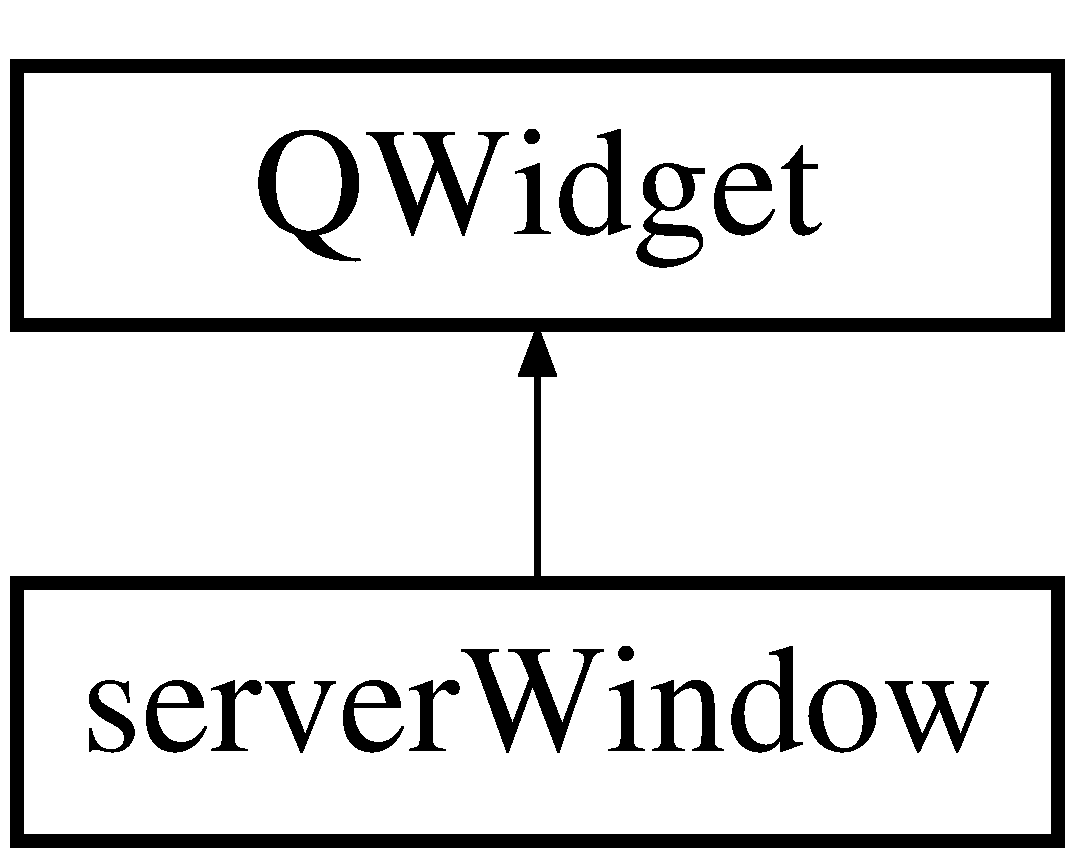
\includegraphics[height=2.000000cm]{classserver_window}
\end{center}
\end{figure}
\subsection*{Signals}
\begin{DoxyCompactItemize}
\item 
\mbox{\Hypertarget{classserver_window_ac4a17bd27c09f0a64382fa130e6cccf7}\label{classserver_window_ac4a17bd27c09f0a64382fa130e6cccf7}} 
void {\bfseries set\+Active\+Widget} (int active\+Widget)
\end{DoxyCompactItemize}
\subsection*{Public Member Functions}
\begin{DoxyCompactItemize}
\item 
\mbox{\hyperlink{classserver_window_a73c38568b8be85b06a301947250c8b58}{server\+Window}} (Q\+Widget $\ast$parent=0)
\begin{DoxyCompactList}\small\item\em \mbox{\hyperlink{classserver_window}{server\+Window}} class constructor. \end{DoxyCompactList}\item 
\mbox{\hyperlink{classserver_window_a8690c73305f40b9b8bc4ee0f42833d4a}{$\sim$server\+Window}} ()
\begin{DoxyCompactList}\small\item\em \mbox{\hyperlink{classserver_window}{server\+Window}} class deconstructor \end{DoxyCompactList}\item 
void \mbox{\hyperlink{classserver_window_a802818e2dd4970c8240efa96bce4c909}{send\+Data}} (Q\+Byte\+Array string)
\begin{DoxyCompactList}\small\item\em sends data from server\+Socket \end{DoxyCompactList}\item 
\mbox{\Hypertarget{classserver_window_af6f4838dce7cf78130b7aa81b3915595}\label{classserver_window_af6f4838dce7cf78130b7aa81b3915595}} 
Q\+Byte\+Array \mbox{\hyperlink{classserver_window_af6f4838dce7cf78130b7aa81b3915595}{get\+Received\+Data}} () const
\begin{DoxyCompactList}\small\item\em received\+Data getter. \end{DoxyCompactList}\end{DoxyCompactItemize}


\subsection{Detailed Description}
\mbox{\hyperlink{classserver_window}{server\+Window}} class is responsible listening to any incoming connection. Class is sending/receiving data over tcp protocol. 

\subsection{Constructor \& Destructor Documentation}
\mbox{\Hypertarget{classserver_window_a73c38568b8be85b06a301947250c8b58}\label{classserver_window_a73c38568b8be85b06a301947250c8b58}} 
\index{server\+Window@{server\+Window}!server\+Window@{server\+Window}}
\index{server\+Window@{server\+Window}!server\+Window@{server\+Window}}
\subsubsection{\texorpdfstring{server\+Window()}{serverWindow()}}
{\footnotesize\ttfamily server\+Window\+::server\+Window (\begin{DoxyParamCaption}\item[{Q\+Widget $\ast$}]{parent = {\ttfamily 0} }\end{DoxyParamCaption})\hspace{0.3cm}{\ttfamily [explicit]}}



\mbox{\hyperlink{classserver_window}{server\+Window}} class constructor. 

Creates new tcp\+Server. 
\begin{DoxyParams}{Parameters}
{\em Q\+Widget} & $\ast$parent \\
\hline
\end{DoxyParams}

\begin{DoxyRetVals}{Return values}
{\em void} & \\
\hline
\end{DoxyRetVals}
\mbox{\Hypertarget{classserver_window_a8690c73305f40b9b8bc4ee0f42833d4a}\label{classserver_window_a8690c73305f40b9b8bc4ee0f42833d4a}} 
\index{server\+Window@{server\+Window}!````~server\+Window@{$\sim$server\+Window}}
\index{````~server\+Window@{$\sim$server\+Window}!server\+Window@{server\+Window}}
\subsubsection{\texorpdfstring{$\sim$server\+Window()}{~serverWindow()}}
{\footnotesize\ttfamily server\+Window\+::$\sim$server\+Window (\begin{DoxyParamCaption}{ }\end{DoxyParamCaption})}



\mbox{\hyperlink{classserver_window}{server\+Window}} class deconstructor 


\begin{DoxyParams}{Parameters}
{\em void} & \\
\hline
\end{DoxyParams}
\begin{DoxyReturn}{Returns}
void 
\end{DoxyReturn}


\subsection{Member Function Documentation}
\mbox{\Hypertarget{classserver_window_a802818e2dd4970c8240efa96bce4c909}\label{classserver_window_a802818e2dd4970c8240efa96bce4c909}} 
\index{server\+Window@{server\+Window}!send\+Data@{send\+Data}}
\index{send\+Data@{send\+Data}!server\+Window@{server\+Window}}
\subsubsection{\texorpdfstring{send\+Data()}{sendData()}}
{\footnotesize\ttfamily void server\+Window\+::send\+Data (\begin{DoxyParamCaption}\item[{Q\+Byte\+Array}]{string }\end{DoxyParamCaption})}



sends data from server\+Socket 


\begin{DoxyParams}{Parameters}
{\em Q\+Byte\+Array} & string \\
\hline
\end{DoxyParams}
\begin{DoxyReturn}{Returns}
void 
\end{DoxyReturn}


The documentation for this class was generated from the following files\+:\begin{DoxyCompactItemize}
\item 
\mbox{\hyperlink{serverwindow_8h}{serverwindow.\+h}}\item 
serverwindow.\+cpp\end{DoxyCompactItemize}

\hypertarget{class_tile}{}\section{Tile Class Reference}
\label{class_tile}\index{Tile@{Tile}}


{\ttfamily \#include $<$tile.\+h$>$}

Inheritance diagram for Tile\+:\begin{figure}[H]
\begin{center}
\leavevmode
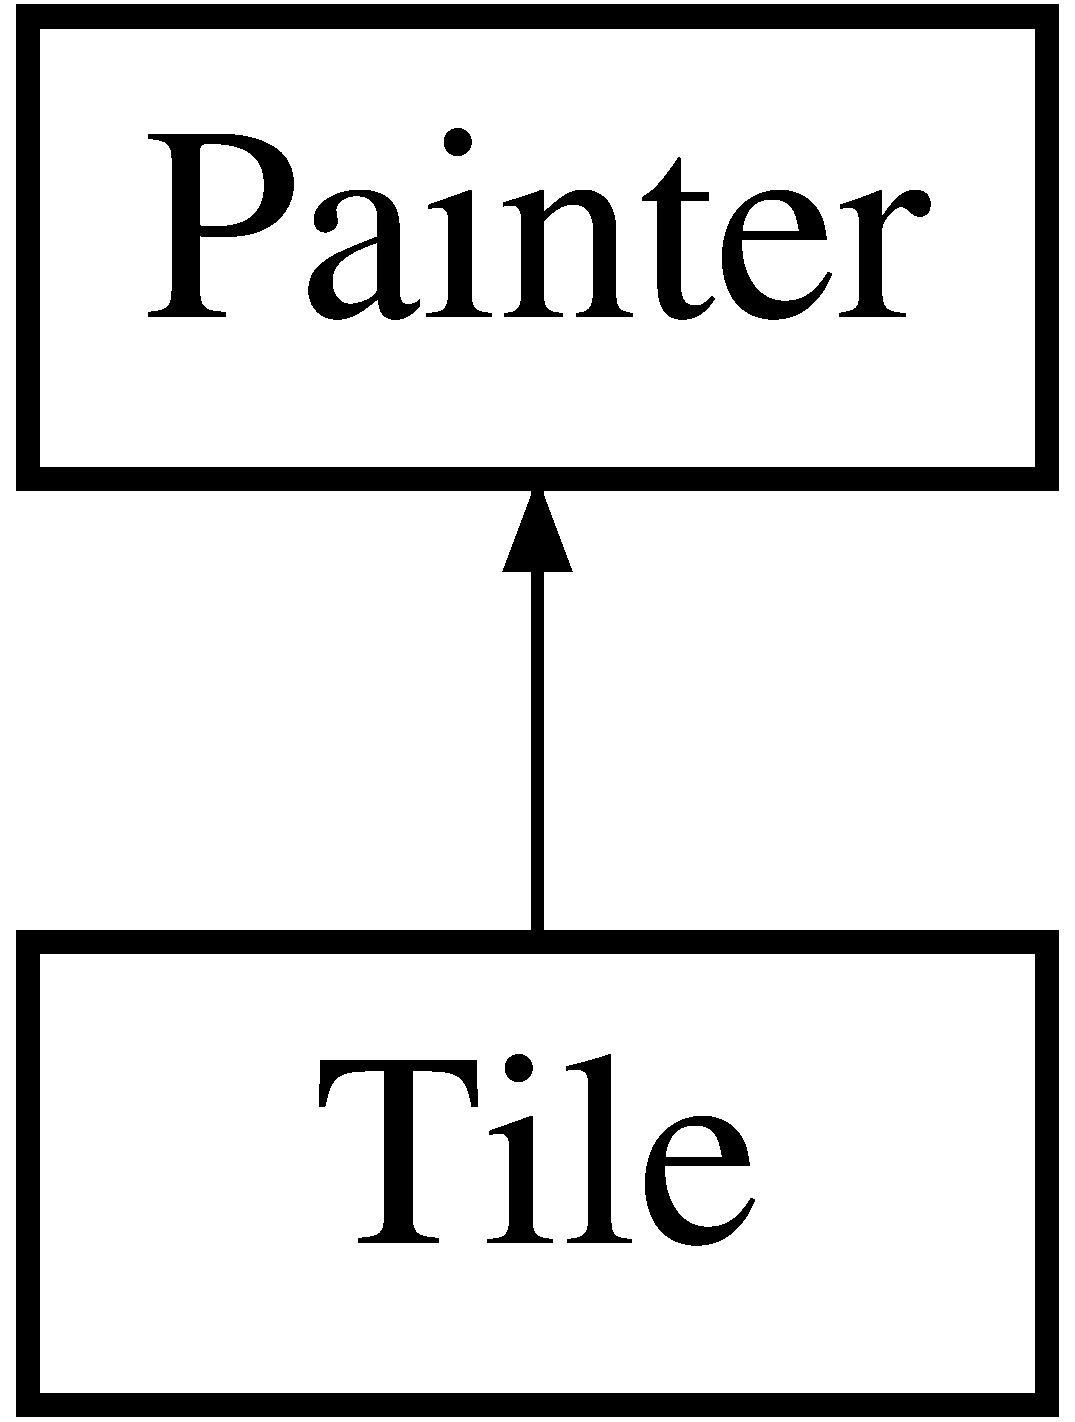
\includegraphics[height=2.000000cm]{class_tile}
\end{center}
\end{figure}
\subsection*{Public Member Functions}
\begin{DoxyCompactItemize}
\item 
\mbox{\hyperlink{class_tile_aeeb5593bb6b75aae2edfcccbc84ab378}{Tile}} ()
\begin{DoxyCompactList}\small\item\em Empty \mbox{\hyperlink{class_tile}{Tile}} class constructor. \end{DoxyCompactList}\item 
\mbox{\hyperlink{class_tile_ab295fb34dca1d8e0b4bf8a3d37ddfbad}{Tile}} (Q\+String pixmap\+Path, int x, int y)
\begin{DoxyCompactList}\small\item\em Overloaded \mbox{\hyperlink{class_tile}{Tile}} class constructor. \end{DoxyCompactList}\item 
\mbox{\Hypertarget{class_tile_a6ae2b82877df3597bec59d3bc99f0f25}\label{class_tile_a6ae2b82877df3597bec59d3bc99f0f25}} 
int \mbox{\hyperlink{class_tile_a6ae2b82877df3597bec59d3bc99f0f25}{get\+Tile\+Type}} () const
\begin{DoxyCompactList}\small\item\em tile\+Type getter. \end{DoxyCompactList}\item 
\mbox{\Hypertarget{class_tile_a987377bd877d64a1d4827638efdd7bfa}\label{class_tile_a987377bd877d64a1d4827638efdd7bfa}} 
void \mbox{\hyperlink{class_tile_a987377bd877d64a1d4827638efdd7bfa}{set\+Tile\+Type}} (int value)
\begin{DoxyCompactList}\small\item\em tile\+Type setter.. \end{DoxyCompactList}\end{DoxyCompactItemize}
\subsection*{Additional Inherited Members}


\subsection{Detailed Description}
\mbox{\hyperlink{class_tile}{Tile}} class transforms x/y coordinates into tiles. Each tile has its own type. 

\subsection{Constructor \& Destructor Documentation}
\mbox{\Hypertarget{class_tile_aeeb5593bb6b75aae2edfcccbc84ab378}\label{class_tile_aeeb5593bb6b75aae2edfcccbc84ab378}} 
\index{Tile@{Tile}!Tile@{Tile}}
\index{Tile@{Tile}!Tile@{Tile}}
\subsubsection{\texorpdfstring{Tile()}{Tile()}\hspace{0.1cm}{\footnotesize\ttfamily [1/2]}}
{\footnotesize\ttfamily Tile\+::\+Tile (\begin{DoxyParamCaption}{ }\end{DoxyParamCaption})}



Empty \mbox{\hyperlink{class_tile}{Tile}} class constructor. 


\begin{DoxyParams}{Parameters}
{\em void} & \\
\hline
\end{DoxyParams}
\begin{DoxyReturn}{Returns}
void 
\end{DoxyReturn}
\mbox{\Hypertarget{class_tile_ab295fb34dca1d8e0b4bf8a3d37ddfbad}\label{class_tile_ab295fb34dca1d8e0b4bf8a3d37ddfbad}} 
\index{Tile@{Tile}!Tile@{Tile}}
\index{Tile@{Tile}!Tile@{Tile}}
\subsubsection{\texorpdfstring{Tile()}{Tile()}\hspace{0.1cm}{\footnotesize\ttfamily [2/2]}}
{\footnotesize\ttfamily Tile\+::\+Tile (\begin{DoxyParamCaption}\item[{Q\+String}]{pixmap\+Path,  }\item[{int}]{x,  }\item[{int}]{y }\end{DoxyParamCaption})}



Overloaded \mbox{\hyperlink{class_tile}{Tile}} class constructor. 

Updates graphics, sets x and y positions. 
\begin{DoxyParams}{Parameters}
{\em Q\+String} & pixmap\+Path, int x, int y \\
\hline
\end{DoxyParams}
\begin{DoxyReturn}{Returns}
void 
\end{DoxyReturn}


The documentation for this class was generated from the following files\+:\begin{DoxyCompactItemize}
\item 
tile.\+h\item 
\mbox{\hyperlink{tile_8cpp}{tile.\+cpp}}\end{DoxyCompactItemize}

\chapter{File Documentation}
\hypertarget{actor_8cpp}{}\section{actor.\+cpp File Reference}
\label{actor_8cpp}\index{actor.\+cpp@{actor.\+cpp}}
{\ttfamily \#include \char`\"{}actor.\+h\char`\"{}}\newline

\hypertarget{clientwindow_8cpp}{}\section{clientwindow.\+cpp File Reference}
\label{clientwindow_8cpp}\index{clientwindow.\+cpp@{clientwindow.\+cpp}}
{\ttfamily \#include \char`\"{}clientwindow.\+h\char`\"{}}\newline
{\ttfamily \#include \char`\"{}ui\+\_\+clientwindow.\+h\char`\"{}}\newline

\hypertarget{gameoptions_8cpp}{}\section{gameoptions.\+cpp File Reference}
\label{gameoptions_8cpp}\index{gameoptions.\+cpp@{gameoptions.\+cpp}}
{\ttfamily \#include \char`\"{}gameoptions.\+h\char`\"{}}\newline
{\ttfamily \#include \char`\"{}ui\+\_\+gameoptions.\+h\char`\"{}}\newline
{\ttfamily \#include $<$Q\+Debug$>$}\newline

\hypertarget{gamewindow_8cpp}{}\section{gamewindow.\+cpp File Reference}
\label{gamewindow_8cpp}\index{gamewindow.\+cpp@{gamewindow.\+cpp}}
{\ttfamily \#include \char`\"{}gamewindow.\+h\char`\"{}}\newline
{\ttfamily \#include \char`\"{}ui\+\_\+gamewindow.\+h\char`\"{}}\newline
\subsection*{Variables}
\begin{DoxyCompactItemize}
\item 
\mbox{\Hypertarget{gamewindow_8cpp_a93c8b2d4401bf4de797e624a7f2feb87}\label{gamewindow_8cpp_a93c8b2d4401bf4de797e624a7f2feb87}} 
\mbox{\hyperlink{class_tile}{Tile}} \mbox{\hyperlink{gamewindow_8cpp_a93c8b2d4401bf4de797e624a7f2feb87}{tile\+Arr}} \mbox{[}M\+A\+P\+\_\+\+T\+I\+L\+E\+S\+\_\+\+W\+I\+D\+TH $\ast$M\+A\+P\+\_\+\+T\+I\+L\+E\+S\+\_\+\+H\+E\+I\+G\+HT\mbox{]}
\begin{DoxyCompactList}\small\item\em Stores tile type of specific array element. \end{DoxyCompactList}\item 
int \mbox{\hyperlink{gamewindow_8cpp_abf9431925aaafbc15219995e08a4ea2f}{non\+Walkable\+Map\+Tiles}} \mbox{[}$\,$\mbox{]} = \{1, 2, 3, 4, 5, 6, 7, 8, 9, 10, 11, 12, 13, 14, 15, 16\}
\begin{DoxyCompactList}\small\item\em Stores all tile numbers on which actor can\textquotesingle{}t be placed. \end{DoxyCompactList}\end{DoxyCompactItemize}


\subsection{Variable Documentation}
\mbox{\Hypertarget{gamewindow_8cpp_abf9431925aaafbc15219995e08a4ea2f}\label{gamewindow_8cpp_abf9431925aaafbc15219995e08a4ea2f}} 
\index{gamewindow.\+cpp@{gamewindow.\+cpp}!non\+Walkable\+Map\+Tiles@{non\+Walkable\+Map\+Tiles}}
\index{non\+Walkable\+Map\+Tiles@{non\+Walkable\+Map\+Tiles}!gamewindow.\+cpp@{gamewindow.\+cpp}}
\subsubsection{\texorpdfstring{non\+Walkable\+Map\+Tiles}{nonWalkableMapTiles}}
{\footnotesize\ttfamily int non\+Walkable\+Map\+Tiles\mbox{[}$\,$\mbox{]} = \{1, 2, 3, 4, 5, 6, 7, 8, 9, 10, 11, 12, 13, 14, 15, 16\}}



Stores all tile numbers on which actor can\textquotesingle{}t be placed. 

\mbox{\hyperlink{class_actor}{Actor}} can\textquotesingle{}t be placed on any wall tile type. 
\hypertarget{ghost_8cpp}{}\section{ghost.\+cpp File Reference}
\label{ghost_8cpp}\index{ghost.\+cpp@{ghost.\+cpp}}
{\ttfamily \#include \char`\"{}ghost.\+h\char`\"{}}\newline

\hypertarget{main_8cpp}{}\section{main.\+cpp File Reference}
\label{main_8cpp}\index{main.\+cpp@{main.\+cpp}}
{\ttfamily \#include \char`\"{}mainwindow.\+h\char`\"{}}\newline
{\ttfamily \#include $<$Q\+Application$>$}\newline
\subsection*{Functions}
\begin{DoxyCompactItemize}
\item 
\mbox{\Hypertarget{main_8cpp_a0ddf1224851353fc92bfbff6f499fa97}\label{main_8cpp_a0ddf1224851353fc92bfbff6f499fa97}} 
int \mbox{\hyperlink{main_8cpp_a0ddf1224851353fc92bfbff6f499fa97}{main}} (int argc, char $\ast$argv\mbox{[}$\,$\mbox{]})
\begin{DoxyCompactList}\small\item\em main function. \end{DoxyCompactList}\end{DoxyCompactItemize}

\hypertarget{mainwindow_8cpp}{}\section{mainwindow.\+cpp File Reference}
\label{mainwindow_8cpp}\index{mainwindow.\+cpp@{mainwindow.\+cpp}}
{\ttfamily \#include \char`\"{}mainwindow.\+h\char`\"{}}\newline
{\ttfamily \#include \char`\"{}ui\+\_\+mainwindow.\+h\char`\"{}}\newline

\hypertarget{pacman_8cpp}{}\section{pacman.\+cpp File Reference}
\label{pacman_8cpp}\index{pacman.\+cpp@{pacman.\+cpp}}
{\ttfamily \#include \char`\"{}pacman.\+h\char`\"{}}\newline

\hypertarget{painter_8cpp}{}\section{painter.\+cpp File Reference}
\label{painter_8cpp}\index{painter.\+cpp@{painter.\+cpp}}
{\ttfamily \#include \char`\"{}painter.\+h\char`\"{}}\newline

\hypertarget{serverwindow_8h}{}\section{serverwindow.\+h File Reference}
\label{serverwindow_8h}\index{serverwindow.\+h@{serverwindow.\+h}}
{\ttfamily \#include \char`\"{}globaltypes.\+h\char`\"{}}\newline
{\ttfamily \#include $<$Q\+Widget$>$}\newline
{\ttfamily \#include $<$Q\+Debug$>$}\newline
{\ttfamily \#include $<$Q\+Tcp\+Server$>$}\newline
{\ttfamily \#include $<$Q\+Tcp\+Socket$>$}\newline
\subsection*{Classes}
\begin{DoxyCompactItemize}
\item 
class \mbox{\hyperlink{classserver_window}{server\+Window}}
\end{DoxyCompactItemize}

\hypertarget{tile_8cpp}{}\section{tile.\+cpp File Reference}
\label{tile_8cpp}\index{tile.\+cpp@{tile.\+cpp}}
{\ttfamily \#include \char`\"{}tile.\+h\char`\"{}}\newline

%--- End generated contents ---

% Index
\backmatter
\newpage
\phantomsection
\clearemptydoublepage
\addcontentsline{toc}{chapter}{Index}
\printindex

\end{document}
